\documentclass[12pt,letterpaper]{article}

\usepackage[hypertexnames=false]{hyperref}
\usepackage{amsmath}
\usepackage{graphicx}
\usepackage{enumerate}
\usepackage{natbib}

% Custom packages
\usepackage{amsthm, amssymb}
\usepackage{booktabs}       % professional-quality tables
\usepackage{algorithm}      % algorithm environment
\usepackage{algpseudocode}
\usepackage{multirow}
\usepackage{sectsty}
\usepackage{tabularx}
\usepackage{tikz}           % vector graphics
\usepackage{bm}             % bold math symbols
\usepackage{xcolor}
\usepackage{microtype}
\usepackage{import}
\usepackage{titling}
\usetikzlibrary{arrows, backgrounds, patterns, matrix, shapes, fit, 
  calc, shadows, plotmarks}

\graphicspath{{./notes/figures/}}


% Custom commands
\let\oldvec\vec
\renewcommand\vec{\bm}
\newcommand{\simfn}{\mathtt{sim}} % similarity function
\newcommand{\truncsimfn}{\underline{\simfn}} % truncated similarity function
\newcommand{\blockfn}{\mathtt{BlockFn}} % blocking function
\newcommand{\distfn}{\mathtt{dist}} % distance function
\newcommand{\valset}{\mathcal{V}} % attribute value set
\newcommand{\entset}{\mathcal{R}} % set of records that make up an entity
\newcommand{\partset}{\mathcal{E}} % set of entities that make up a partition
\newcommand{\1}[1]{\mathbb{I}\!\left[#1\right]} % indicator function
\newcommand{\euler}{\mathrm{e}} % Euler's constant
\newcommand{\dblink}{\texttt{\upshape \lowercase{d-blink}}} % Name of scalable Bayesian ER model
\newcommand{\blink}{\texttt{\upshape \lowercase{blink}}} % Name of original Bayesian ER model
\def\spacingset#1{\renewcommand{\baselinestretch}%
  {#1}\small\normalsize} \spacingset{1}

\newtheorem*{remark}{Remark}
\newtheorem{proposition}{Proposition}
\newtheorem*{definition}{Definition}

% DON'T change margins - should be 1 inch all around.
\addtolength{\oddsidemargin}{-.5in}%
\addtolength{\evensidemargin}{-.5in}%
\addtolength{\textwidth}{1in}%
\addtolength{\textheight}{1.3in}%
\addtolength{\topmargin}{-.8in}%

\sectionfont{\large\nohang\centering\MakeUppercase}

\title{Efficient and Scalable Bipartite Matching with Fast Beta Linkage  (fabl)}
\author{Brian Kundinger\textsuperscript{a} \and
  Jerome Reiter\textsuperscript{a} \and 
  Rebecca C.~Steorts \textsuperscript{b}}
\date{
 \textsuperscript{a} Department of Statistical Science, Duke University \\
 \textsuperscript{b} Department of Statistical Science and Computer Science, Duke University\\Principal Mathematical Statistician, United States Census Bureau\\[2ex]
  \today}

\begin{document}
\maketitle

\bigskip
\begin{abstract}
Abstract
\end{abstract}


\noindent%
{\it Keywords:} record linkage, Bayesian methods, paralellized computing, streaming algorithms

\newpage
\spacingset{1.5}

\section{Introduction}
\label{sec:introduction}

Record linkage is the task of identifying
duplicate records across multiple data sources. In many cases, this identification is itself the goal of an analysis, as in estimating human rights atrocities from disparate data sources, or linking voter information across election years. In others, we seek to perform some other statistical procedure, such as survival analysis or regression, using linked datasets, and one must  propagate linkage uncertainty into the subsequent analysis. 

Record linkage is straightforward when provided unique identifiers or highly reliable information, but becomes difficult when data sources are plagued with error. This motivates the use of probabilistic record linkage techniques that are able to model the reliability of the information and which are more robust to errors than are deterministic methods. Unfortunately, probabilistic record linkage is computationally intense, and many entity resolution tasks are large in nature,
motivating the search for scalable and efficient record linkage techniques. 

Most record linkage techniques are based the seminal \citep{fs}, which formalized the methods outlined by \citep{newcombe}. This method creates comparison vectors for each pair of records in the data, and independently classifies those pairs as a match or a non-match. Though this independence is usually not reasonable, it is appealing for its mathematical simplicity and relative computational ease. Several authors have elaborated on this approach by including hierarchical structure on model parameters, aiding classification through regression to incorporate covariates, establishing joint models for linkage and analysis, and more \citep{larsen2005}, \citep{hu2017}, \citep{hof2017}. Importantly, \citep{enamorado2019} modified the Fellegi-Sunter method with innovative hashing techniques, greatly expanding the scalability of the independent classification approach. 

Despite the appeal of independent classification, it often leads to linkage decisions that do not enjoy transitive closure, and ignores that fact that we are often in scenarios where we know one record in one file has at most one match in another file. This setting is known as bipartite matching, and has received much less attention in the literature. \citep{sadinle2017} developed a prior distribution on the space of bipartite matchings such that his method, known as Beta Record Linkage (BRL), resulted in one-to-one matchings without any need for post-processing. However, BRL was even more computationally intensive than the original Fellegi-Sunter method, making it infeasible for large linkage tasks. 

In this paper, we propose an extension to the \texttt{BRL} method proposed by \citep{sadinle2017} for this very end.  We increase the speed of the \texttt{BRL} procedure through a modification to the model specification that allows for parallel computing of the linkage parameter, and use hashing techniques to hasten calculations and reduce computational complexity. Additionally, we introduce storage efficient indexing (SEI), and a data partitioning approach to make the method amenable to large linkage tasks. To recognize the lineage from the original \texttt{BRL} method, we name our method \emph{Fast Beta Linkage} (\texttt{fabl},
pronounced ``fable'')

In what follows, Section~\ref{sec:related} describes previous work in record linkage that lays the foundation for our method, Section~\ref{sec:model}
3 provides our model and the Gibbs sampler used for posterior inference,
and Sections~\ref{sec:efficiency} and~\ref{sec:efficient-posterior} describe strategies used for more efficient and scalable
implementation. Then, Section~\ref{sec:simulations} demonstrates the accuracy and speed of
out method through two simulation studies, and Section~\ref{sec:case-studies} reveals
interesting properties of the method through a case study of El
Salvadoran casualty records. Lastly, Section~\ref{sec:discussion} is a discussion that highlights open
questions in the record linkage literature and motivates future work.


\section{Related work}
\label{sec:related}

\paragraph{Fellegi and Sunter Method}
Most record linkage techniques are derived from the seminal \citep{fs} paper "A Theory for Record Linkage". The defining
characteristic of their approach was to transform the sets of records,
which often contain text data that is difficult to model, into sets of
comparison vectors governed by parameters that can be more easily
estimated. Concretely, if files \(A\) and \(B\) have \(n_A\) and \(n_B\)
records respectively, and if the files share \(F\) fields in common upon
which to base the linkage, the Fellegi and Sunter approach generates an
\(n_A n_B \times F\) matrix \(\Gamma\), which contains similarity scores
between each pair of records across datasets. We say \(\gamma_{ij}\) is
the comparison vector for record \(i \in A\) and record \(j \in B\),
with \(\gamma_{ij}^f \in \{1, \ldots, L_f\}\) providing their similarity
score on the \(f^{th}\) field. For ease of modeling and computation, we
restrict these similarity scores to be discrete, ordinal variables, and
the construction of these is left to the modeler. We adopt the
convention that \(\gamma_{ij}^f = 1\) corresponds to the highest level
of agreement and \(\gamma_{ij}^f = L_f\) corresponds to the lowest. It
is common to use use binary 1-2 variables to indicate exact matching,
and 1-2-3 variables to provide an option for partial matching. For text
data, we calculate similarity based on Levenstein distance or some other
text similarity score, and bin these scores to integers for use in the
model. \citep{jaro1989} provided guidelines for appropriate binning for the
comparison vectors, but details of implementation are generally context
specific.

The likelihood in the original Fellegi Sunter model is a mixture model
through which each record pair is independently classified as a match or
nonmatch. This independent classification often leads to sets of matches
that break expectations of transitivity, which is undesirable. Although
\citep{jaro1995} devised an procedure to reduce a set of conflicting matches to the
mostly likely set of one-to-one matchings, the abundance of false
matches can bias the estimation of other parameters of the model, and ultimately leads to poor linkage performance. 

\citep{sadinle2017} uses the same comparison vector approach as Fellegi and Sunter, but proposed a prior distribution for the set of matches that strictly enforced one-to-one matching without the need for any post-hoc processing procedures. Specifically, in each iteration of his Gibbs sampler, he considers each record \(j\in B\), removes from consideration the records \(i\in A\) that have already been matched, and then samples a potential link. This leads to a sampler that is significantly more accurate than the standard Fellegi-Sunter approach. However,
accounting for these dependencies throughout the linkage process is
computationally burdensome, leaving \texttt{BRL} only suitable for small
to moderate linkage problems.

%Outside of the Fellegi-Sunter framework, some researchers have developed
%methods that model the data directly, not a derived set of comparison
%vectors. As an early example,  produced \texttt{blink}, which had the advantage of a computational complexity
%that grew linearly with the data (as opposed to quadratically within
%Fellegi Sunter), but was plagued with slow mixing times and was unable
%to incorporate text data. Later, Steorts et al 2020 improved on this
%method with \texttt{dblink}, which was able to simulate text data within
%its Gibbs sampler by drawing from an empirical distribution, and
%remedied its slow mixing through a probabilistic blocking approach.
%However, this method remains computationally intensive and requires
%distributed computing to manage even moderate linkage problems in
%acceptable time. These methods perform entity resolution over arbitrary numbers of datasets with arbitrary amounts of duplication and fall outside the Fellegi-Sunter framework, so we do not discuss them further here. 

\section{A scalable model for Bayesian Record Linkage}
\label{sec:model}

In this section, we propose a statistical model suitable for efficient computation in large linkage tasks. Denote two files as \(A\) and \(B\), with \(n_A\) and \(n_B\) records
respectively, and with records indexed as \(i \in \{1, \ldots, n_A\}\)
in \(A\) and \(j \in \{1, \ldots, n_B\}\) in \(B\). Without loss of
generality, label the files such that \(n_A \geq n_B\). We assume there
are no duplicates within files, only across. For each record pair under
consideration, we generate a comparison vector
\(\boldsymbol{\gamma}_{ij} = \{\gamma_{ij}^1, \ldots, \gamma_{ij}^F\}\),
where \(F\) is the number of fields used in the linkage and each
\(\gamma_{ij}^f\) takes on a value \(l \in \{1, \ldots, L_f\}\)
indicating the level agreement between the two records on a specified
field.

To indicate matching status, we adopt the \emph{linkage structure
	parameter} \(\mathbf{Z} = (Z_1, \ldots, Z_{n_B})\) from Sadinle 2017,
defined as \[Z_j=\begin{cases} 
	i,  & \text{if records } i\in A \text{ and } j\in B \text{ refer to the same entity}; \\
	n_A + 1,  & \text{if record } j\in B \text{ does not have a match in file } A; \\
\end{cases}\] This parameter is vector of length $n_B$, providing more memory efficient storage for the
linkage information than a \(n_A \times n_B\) sparse matrix of
indicators.

Following the Fellegi Sunter framework, we define
\(m^{fl}:= P(\gamma_{ij}^f = l |Z_j = i)\) to be the probability of
observing agreement level \(l\) in field \(f\) for records \(i\) and
\(j\) given that the records are a match, and similarly define
\(u^{fl}:= P(\gamma_{ij}^f = l |Z_j \neq i)\), for non-matches. We also
adopt Fellegi and Sunter's conditionally independent fields assumption
that the level of agreement on one field is independent of the level of
agreement on another. Though this assumption is often not reasonable
(for example, two individuals of a different genders are more likely to have different names than two individuals of the same gender),
but it is common within the record linkage literature and generally
leads to models that perform well in practice; see discussion for
further remarks. Lastly, we define \(\lambda\) to be the (marginal)
probability that some record \(j \in B\) has a match in \(A\).

%Wherever possible, we reserve superscripts for denoting field and level,
%while reserving subscripts for record indices. For example,
%\(\mathbf{m}^f = (m^{f1}, \ldots, m^{fL_f})\) is the probability
%distribution governing field \(f\) for matching records, and
%\(\mathbf{m}_{ij}= \prod_{f=1}^{F}\prod_{l=1}^{L_f} \left(m^{fl}\right)^{\mathbf{1}_{\gamma_{ij}^f = l}} = P(\boldsymbol{\gamma}_{ij}|Z_j = i)\)
%is product of the relevant of the appropriate \(\mathbf{m}\) parameters
%for record pair \((i,j)\). We hope that these conventions avoid
%overloaded notation in the likelihood and subsequent derivations.

\hypertarget{model-specification}{%
	\subsection{Model Specification}
	\label{model-specification}}

For fields \(f \in \{1, \ldots, F\}\) and levels
\(l\in \{1, \ldots, L_f\}\) we adopt the following likelihood and prior
distributions.

%\[P(\Gamma|\mathbf{Z}, \mathbf{m}, \mathbf{u}, \lambda) =\prod_{j=1}^{n_B}  \prod_{i=1}^{n_A}\mathbf{m}_{ij}^{\mathbf{1}_{z_j = i}}\mathbf{u}_{ij}^{\mathbf{1}_{z_j \neq i}}\]

$$P(\Gamma|\mathbf{Z}, \mathbf{m}, \mathbf{u}) = \prod_{j=1}^{n_B}  \prod_{i=1}^{n_A}\left[ \prod_{f=1}^{F}\prod_{l=1}^{L_f} m_{fl}^{I(Z_j = i)}u_{fl}^{I(Z_j \neq i)}\right]^{I(\gamma_{ij}^f = l)}$$

\[\mathbf{m^{f}} \sim \text{Dirichlet}(\alpha^{f1}, \ldots, \alpha^{fL_f})\]
\[\mathbf{u^{f}} \sim \text{Dirichlet}(\beta^{f1}, \ldots, \beta^{fL_f})\]
\[Z_j | \lambda =
\begin{cases} 
	\frac{1}{n_A}\lambda  & z_j \leq n_A; \\
	1-\lambda &  z_j  = n_A + 1 \\
\end{cases}\]

\[\lambda \sim \text{Beta}(\alpha_{\lambda}, \beta_{\lambda}) \] The
prior for \(Z_j\) has equal probability of matching to all records
\(i\in A\), and non-matching probability governed by \(\lambda\).
Therefore a \(\lambda \sim \text{Beta}(1, 1)\) corresponds to a prior
belief that nonmatches and matches are equally likely, and a
\(\lambda \sim \text{Beta}\left(1, \frac{1}{n_A}\right)\) prior
corresponds to a uniform prior on the labeling of \(\mathbf{Z}\).

Here the reader should the relationship between our proposed model and
that of Sadinle 2017. In his model, Sadinle constructs a prior
distribution on the entire \(\mathbf{Z}\) vector, which induces a Gibbs
sampler that strictly enforces one-to-one matching. In particular, this
sampler removes previously matches records from the set of candidate
records when sampling \(Z_j\), creating a dependency that makes the
sampler \emph{inherently serial}. We however use independent priors for
each \(Z_j\), creating a sampler that is \emph{perfectly parallelizable}, allowing for significant computational gains. More
importantly, since only the agreement pattern of \(Z_j\) is used for
calculations within the Gibbs sampler, and not the particular record
label, we can conduct this sampling only at the level of the unique
agreement patterns, offering even more computational savings. In doing
so however, we thereby weaken the one-to-one requirement from
\texttt{BRL}; our sampler does ensure that each record in \(B\) can be
matched to at most one record in \(A\), but allows for the possibility
that multiple records in \(B\) match to the same record in \(A\). We then resolve these contradictions through a straightfoward post-processing step. We
explore the ramifications of this distinction with the El Salvador case
study.

\hypertarget{posterior-sampling}{%
	\subsection{Gibbs Sampler}
	\label{gibbs_sampling}}
We work with the following factorization of the joint posterior distribution:

\begin{align*}
p(\mathbf{Z}, \mathbf{m}, \mathbf{u}, \lambda|\Gamma) &\propto p(\Gamma|\mathbf{Z}, \mathbf{m}, \mathbf{u}) p(\mathbf{Z} | \lambda) p(\mathbf{m}, \mathbf{u}) p(\lambda) \\
&\propto \prod_{j=1}^{n_B}  \prod_{i=1}^{n_A}\left[ \prod_{f=1}^{F}\prod_{l=1}^{L_f} m_{fl}^{I(Z_j = i)}u_{fl}^{I(Z_j \neq i)}\right] \\
&\times  \prod_{f=1}^{F}\prod_{l=1}^{L_f} m_{fl}^{\alpha_{fl} - 1}  \times\prod_{f=1}^{F}\prod_{l=1}^{L_f} u_{fl}^{\beta_{fl} - 1} \\
&\times \prod_{j=1}^{n_B} \left[I(Z_j \leq n_A)\frac{1}{n_A}\lambda + I(Z_j = n_A + 1)(1 - \lambda)\right]
\end{align*}
This factorization leads to following Gibbs Sampler:

\underline{Sample $\mathbf{m}^{(s+1)}$ $\mathbf{u}^{(s+1)}|\Gamma, \mathbf{Z}^{(s)}$:}
The \(\mathbf{m}\) and \(\mathbf{u}\) parameters are updated through
standard multinomial-dirichlet mechanics. Thus we have

\[\mathbf{m}_f|\mathbf{Z}, \Gamma \sim \text{Dirichlet}(\alpha_{f1}(\mathbf{Z}), \ldots, \alpha_{fL_f}(\mathbf{Z}))\]
\[\mathbf{u}_f|\mathbf{Z}, \Gamma \sim \text{Dirichlet}(\beta_{f1}(\mathbf{Z}), \ldots, \beta_{fL_f}(\mathbf{Z}))\]
where
\(\alpha_{fl}(\mathbf{Z})= \alpha_{fl} + \sum_{i,j} I(\gamma_{ij}^f = l) I(z_j = i)\)
and
\(\beta_{fl}(\mathbf{Z})= \beta_{fl} + I(\gamma_{ij}^f = l) I(z_j \neq i)\).

\underline{Sample $\lambda^{(s+1)}|\mathbf{Z}^{(s)}$:} As a function of
\(\lambda\), the linkage structure parameter \(\mathbf{Z}\) is sequence
of successes (when \(z_j < n_A + 1\)) and failures (when
\(z_j = n_A + 1\)), and therefore
\(p(\mathbf{Z}|\lambda) = \mathcal{L}(\lambda|\mathbf{Z})\) is
determined only by the number of duplicates
\(D = \sum_{i=1}^{n_B}\mathbf{1}_{z_j < n_A + 1}\) encoded by
\(\mathbf{Z}\). Thus we have

\[p(\lambda | \mathbf{Z}) \propto p(\mathbf{Z}|\lambda)p(\lambda)\]
\[\propto \lambda^D (1-\lambda)^{n_B - D} \lambda^{\alpha_{\lambda} -1} (1-\lambda)^{\beta_{\lambda} -1}\]
\[ \propto \lambda^{D + \alpha_{\lambda} - 1} (1-\lambda)^{n_B - D + \beta_{\lambda} -1}\]
\[\implies \lambda^{(s+1)}|\mathbf{Z}^{(s+1)} \sim \text{Beta}(D + \alpha_{\lambda}, n_B - D + \beta_{\lambda})\]

\underline{Sample $\mathbf{Z}^{(s+1)}|\Gamma, \mathbf{m}^{(s+1)}, \mathbf{u}^{(s+1)}, \lambda^{(s+1)}$:}
Because we sample \(Z_j\) independently of all other \(Z_{j'}\), we use
only the full conditional for an individual \(Z_j\). Let \(\Gamma_{.j}\)
denote the set of \(n_A\) comparison vectors with \(j \in B\), and note
that as a function of \(Z_j\), the likelihood
\(p(\Gamma_{.j}|Z_j, \mathbf{m}, \mathbf{u}) = \mathcal{L}(Z_j|\Gamma_{.j}, \mathbf{m}, \mathbf{u})\)
is a discrete distribution with probabilities proportional to

\begin{align*}
	p(\Gamma_{.j}|Z_j = z_j, \mathbf{m}, \mathbf{u}) &\propto \prod_{i=1}^{n_A}\left[\prod_{f=1}^{F}\prod_{l=1}^{L_f} m_{fl}^{I(Z_j = i)}u_{fl}^{I(Z_j \neq i)}\right]^{I(\gamma_{ij}^f = l)}\\
	&\propto \prod_{i=1}^{n_A}\left(\prod_{f=1}^{F}\prod_{l=1}^{L_f} \frac{m_{fl}}{u_{fl}}\right)^{I(z_j = i, \gamma_{ij}^f = l)} \\
	&=
	\begin{cases} 
		w_{ij}  & z_j \leq n_A; \\
		1 &  z_j  = n_A + 1 \\
	\end{cases}\\
\end{align*}

where
\(w_{ij} = \left(\frac{\prod_{f=1}^{F}\prod_{l=1}^{L_f} m_{fl}}{\prod_{f=1}^{F}\prod_{l=1}^{L_f} u_{fl}}\right)^{I(\gamma_{ij}^f = l)} = \frac{P(\boldsymbol{\gamma_{ij}}|Z_j = i)}{P(\boldsymbol{\gamma_{ij}} |Z_j \neq i)}\).
The interested reader should note that these are precisely the
likelihood ratios used in the Fellegi-Sunter model to classify matches
and non-matches, and we therefore refer to \(w_{ij}\) as the
\emph{Fellegi Sunter weights}.

With the likelihood in this form, we can derive the full conditional
\[p(Z_j|\Gamma_{.j}, \mathbf{m} ,\mathbf{u}, \lambda) \propto p(\Gamma_{.j}| Z_j, \mathbf{m} ,\mathbf{u}) P(Z_j|\lambda)\]

\[\propto \left(\sum_{i=1}^{n_A}w_{ij}\mathbf{1}_{z_j = i} + \mathbf{1}_{z_j = n_A + 1}\right)\left(\lambda\sum_{i=1}^{n_A}\frac{1}{n_A}\mathbf{1}_{z_j = i} + (1-\lambda)\mathbf{1}_{z_j = n_A + 1}\right)\]
\[= \frac{\lambda}{n_A}\sum_{i=1}^{n_A}w_{ij}\mathbf{1}_{z_j = i} + (1-\lambda)\mathbf{1}_{z_j = n_A + 1} \]
\[ \implies Z_j^{(s+1)} | \mathbf{m}, \mathbf{u}, \Gamma, \lambda \propto
\begin{cases} 
	\frac{\lambda}{n_A}w_{ij}   & z_j \leq n_A; \\
	1-\lambda &  z_j  = n_A + 1 \\
\end{cases}\]

In order to make fair comparisons against the \citep{sadinle2017} model, we
integrate over the posterior of \(\lambda\) and rearrange terms to
produce the final full conditional:

\[p\left(Z_j^{(s+1)}  = i| \mathbf{m}, \mathbf{u}, \mathbf{Z^{(s)}}\right) \propto
\begin{cases} 
	w_{ij}  & i \leq n_A; \\
	n_A \frac{n_B - D + \beta_{\lambda}}{D + \alpha_{\lambda}} & i  = n_A + 1 \\
\end{cases}\]

\hypertarget{bayes-estimate}{%
	\subsection{Bayes Estimate}
	\label{bayes-estimate}}

We calculate a Bayes estimate \(\hat{\mathbf{Z}}\) for the linkage
parameter \(\mathbf{Z}\) by assigning different positive losses to
different types of errors, and minimizing posterior expected loss. We
adopt the loss function proposed in Sadinle 2017, in which
\(\hat{Z}_j \in \{1, \ldots, n_A + 1, R\}\), with \(R\) representing the
option to leave the matching undetermined by the model. Specifically, we
minimize the quantity
\(L(\hat{\mathbf{Z}}, \mathbf{Z}) = \sum_{j=1}^{n_B} L(\hat{Z_j}, Z_j)\)
where

\[L(\hat{Z_j}, Z_j)=\begin{cases} 
	0  & \text{if } Z_j = \hat{Z_j}; \\
	\theta_R,  & \text{if } \hat{Z_j} = R; \\
	\theta_{10},  & \text{if } Z_j \leq n_A,\hat{Z_j} = n_A + 1 ; \\
	\theta_{01},  & \text{if } Z_j = n_A + 1,\hat{Z_j} \leq n_A ; \\
	\theta_{11},  & \text{if } Z_j, \hat{Z}_j \leq n_A, Z_j \neq \hat{Z_j} ; \\
\end{cases}\] Here, \(\theta_R\) is the loss from not making a decision
on the linkage status, \(\theta_{10}\) is the loss from a false
non-match, \(\theta_{01}\) is the loss from a false match, and
\(\theta_{11}\) is the loss from the special case of a false match in
which the record has a true match other than the one estimated by the
model. This loss function leads to closed form decision rules for
minimizing posterior expected loss. In this paper, we adopt losses
\(\theta_R = \infty, \theta_{10} = 1, \theta_{01} = 1, \theta_{11} = 2\),
inducing the intuitive decision rule

\[\hat{Z}_j =\begin{cases} 
	i,  & \text{if } P(Z_j = i |\Gamma) > \frac{1}{2}; \\
	0,  & \text{otherwise} ; \\
\end{cases}\]

For a more in-depth explanation of this function and the induced Bayes
estimate, see \citep{sadinle2017}.

Since our Gibbs procedure does not strictly enforce one-to-one matching,
it is possible for the final Bayes estimate to link multiple records in
\(B\) to one record in \(A\). The modeler can either report both such
matches (with their respective posterior match probabilities), or
resolve these conflicts by accepting only the match with highest
posterior probability. A similar approach can be see in the most probable maximal matching sets used by \citep{steorts_2013} to match records to latent entities. Such a resolution procedure indeed is equivalent
to minimizing posterior risk under the restriction of one-to-one
matching, and as thus theoretically justified within the Bayesian
framework.

\section{Efficient and Scalable Implementation}
\label{sec:efficiency}
Broadly speaking, we increase our computational efficiency by
recognizing that record pairs contribute to posterior calculations only
through the agreement pattern of the \(\gamma_{ij}\) vector. Let
\(\mathcal{H}\) be the set of unique agreement patterns in the data, let
\(P = |\mathcal{H}|\) denote the total number of unique agreement
patterns.  Note that \(P\) is bounded above by \(\prod_{f=1}^F L_f\), and
that this bound does not scale with \(n_A\) or \(n_B\). Prior to
processing the data, we identify all \(P\) patterns in \(\mathcal{H}\)
and enumerate them \(h_1, \ldots, h_P\), and map record pairs to this hashed value. When the \((i,j)\) pair
exhibits the \(p^{th}\) agreement pattern, we say \((i,j) \in h_p\).
Wherever possible, we conduct calculations over these \(P\) agreement
patterns rather than the \(n_A \times n_B\) record pairs. Some of these techniques are similar to those used by \citep{enamorado2019} to produce \texttt{fastlink}, a fast a scalable implementation of the Fellegi-Sunter model, and others have been created here for our particular context. 

\hypertarget{data-representation-hashing-and-storage}{%
	\subsection{Data Representation, Hashing, and
		Storage}\label{data-representation-hashing-and-storage}}

We first hash record pairs of the same agreement pattern to unique integer values. \citep{enamorado2019} accomplished this efficiently through the hashing function
$$\tilde{\gamma}_{ij} = \sum_{f = 1}^F I(\gamma_{ij}^f > 0)2^{\gamma_{ij}^f + I(k>1)\sum_{e=1}^{k-1}(L_e -1)}$$
This function maps each agreement pattern to a unique integer, allowing us to store a scalar quanity instead of an entire vector for each record pair. For computational ease, we then map these integers to sequential integers from 1 to P. 

The classic Fellegi Sunter method represents the \(\gamma_{ij}\)
comparison as a vector of length \(F\), with each component
\(\gamma_{ij}^f\) taking on values in \(\{1, \ldots, L_f \}\). To ease
computations, we instead use a one hot encoding of the comparison vector. For example, if
\(L_1 = L_2 = 2\) and \(L_3 = 3\), then \(\gamma_{ij} = (2, 1, 3)\)
under the classical framework becomes
\(\gamma_{ij} = (0, 1, 1, 0, 0, 0, 1)\) under our framework. This is a
bijective transformation that does not change the meaning of the data,
but this representation eases calculations and posterior updates. This is also the form the data takes in the \texttt{BRL} package in \texttt{R}. 

In the classic Fellegi Sunter framework, \(\Gamma\) is a
\(n_A n_B \times F\) matrix, with each row providing the comparison
vector for a different \((i,j)\) pair. In contrast, we do not store
these comparison vectors themselves, but instead only the hashed value $h_p$
corresponding to the agreement pattern of the \((i, j)\) pair. We store
this information in a nested list \(\tilde{\Gamma}\) where the
\(p^{th}\) component of the \(j^{th}\) list contains a vector of records
in \(A\) that share agreement pattern \(p\) with record \(j \in B\). For
each \(p\), we also calculate
\(H_p = \sum_{i=1}^{n_A}\sum_{j=1}^{n_B} \mathbf{1}_{(i,j) \in h_p}\),
the total instances of agreement pattern \(p\) throughout the data, and
also for each \(j\), we calculate
\(H_{p_j} = \sum_{i=1}^{n_A} \mathbf{1}_{{(i,j) \in h_p}}\) the
instances of agreement pattern \(p\) among the comparison vectors
between record \(j \in B\) and each of the \(n_A\) records in \(A\).

The hashing procedure described above considerably reduces the memory
needed to store the comparison information: instead of storing
\(n_A \times n_B\) comparison vectors, which are relatively long under
either the Fellegi Sunter or our modified framework, we only store the
\(P\) unique vectors, and then \(n_A \times n_B\) scalar quantities
relating record pairs to those vectors. However, even storing these
\(n_A \times n_B\) scalar labels can become burdensome with large data.
Worse, the overwhelming majority of these labels relate to record pairs
that are clear non-matches.

To address this, we propose a new strategy called \emph{storage	efficient indexing} (SEI). In standard indexing, the modeler decides a
certain criteria that they expect all true matching pairs to satisfy,
and a priori label any record pairs that do not meet that criteria as
non-matching. For example, one might only consider pairs with a certain
similarity score on a field deemed to be important (like first name), or
only pairs with exact matching on a specified number of fields. While
generally chosen to be be quite loose, establishing these criteria
requires knowledge of the problem and invites room for human error. We
propose a method of reducing the comparison space (and reducing storage
requirements) without these drawbacks. Note that all records of the same
agreement pattern have the same probability when sampling \(Z_j\).
Therefore we know that records belonging to an \(h_p\) such that
\(H_{p_j}\) is large are very unlikely to be sampled consistently enough
to be deemed a match through the Bayes estimate, even without
considering the form of the agreement pattern itself.

In SEI, rather than store all of these unlikely record labels, we choose
to store only a small number \(R\) of them. Posterior calculations still
attribute the appropriate weight to all records through the summary
statistics \(H_p\), and \(H_{p_j}\). Rather than storing
\(n_A \times n_B\) record labels, SEI allows us to store at most
\(n_B \times P \times R\) labels, regardless of how large \(n_A\) is.

Lastly, for large data, we can partition the two datasets \(A\) and
\(B\) into smaller blocks \(\{A_m\}\) and \(\{B_m\}\) for more
manageable computations. On a single machine, we can read-in data
sequentially, conduct hashing, compress information through SEI, and
delete the original data from memory before continuing with the next
chunk of data. With multiple cores or multiple machines, this can be
done in parallel. Thus the combination of hashing, SEI, and partitioning
allows us to conduct linkage tasks over much larger datasets.


\section{Efficient Posterior Inference}\label{sec:efficient-posterior}

\underline{Updating $\mathbf{m}$ and $\mathbf{u}$:} After receiving
matching statuses from \(\mathbf{Z}\), the Sadinle method calculates
\(\alpha_{fl}(\mathbf{Z})\) and \(\beta_{fl}(\mathbf{Z})\) for each
field and level. This constitutes \(2 \times \sum L_f\) many summations
over \(n_A \times n_B\) quantities, and becomes computationally
burdensome with large data. In contrast, we recognize that each unique
agreement pattern contributes to the posterior \(\alpha(\mathbf{Z})\)
and \(\beta(\mathbf{Z})\) vectors in the same way. In fact, if we denote
\(H_p^m = \sum_{j=1}^{n_B} \mathbf{1}_{(Z_j, j) \in h_p}\) to be the
number of matching record pairs with agreement pattern \(p\), then the
contribution of pairs of pattern \(p\) to the \(\alpha(\mathbf{Z})\)
vector is simply \(H_p^m \times h_p\). Thus our posterior update for the
\(\alpha\) vector is simply
\(\alpha(\mathbf{Z}) = \alpha_0 + \sum_{p=1}^P H_p^m \times h_p\). Then,
we can easily calculate \(H_p^u\), the number of nonmatching record
pairs of agreement pattern \(p\), by subtracting the number of matching
pairs from the total present in the data; that is
\(H_p^u = H_p - H_p^m\). From this, we can update our \(\beta\)
parameter through
\(\beta(\mathbf{Z}) = \beta_0 + \sum_{p=1}^P H_p^u \times h_p\). Note
that these constitute \(P\) many summations over \(n_B\) quantities, and
thus avoid the \(n_A \times n_B\) summation from the original method.

\underline{Updating $\mathbf{Z}$:} Although sampling \(Z_j\) from a the
full conditional provided earlier is conceptually straightforward, it
becomes computational burdensome when \(n_A\) is larger. The reader can
confirm that sampling a value from a large set of unequal probabilities
becomes difficult in most programming languages. To speed up
computation, we break this sampling step into two simpler steps. First,
we calculate the Fellegi Sunter weight \(w_{p}\) associated with each
unique pattern and sample the agreement pattern between \(j\) and its
potential match. Second, we sample the record label uniformly among
records associated with that agreement pattern for that particular
\(j\in B\). More concretely, define \(h(Z_j)\) to be the agreement
pattern between \(j\) and its potential match, and say
\(h(Z_j) = h_{P+1}\) when \(Z_j = n_A + 1\). Then,

\[P\left(h\left(Z_j^{(s+1)}\right) = p | \mathbf{m}, \mathbf{u}, \mathbf{Z^{(s)}}\right) \propto
\begin{cases} 
	w_{p}\times H_{p_j}  & p \leq P; \\
	n_A \frac{n_B - D + \beta_{\lambda}}{D + \alpha_{\lambda}} &   p = P + 1 \\
\end{cases}\]
\[P\left(Z_j^{(s+1)} = i\bigg|\;\; h\left(Z_j^{(s+1)}\right) = p\right) = \begin{cases} 
	\frac{1}{H_{p_j}} & (i, j) \in h_p \\
	0 & \text{otherwise} \\
\end{cases}\]

Lastly, we recognize that all posterior updates are governed by the
agreement patterns of the record pairs rather than the record labels
themselves. Thus we complete the entire Gibbs procedure first at the
level of the \(P\) agreement patterns with the first equation above.
After, we can back-fill the records corresponding to the agreement
patterns through the second equation. Sampling uniformly is
computationally simple even for large sets of candidate records, but this
step can also be parallelized when working with large data.

To aid the reader, we provide summary of the \texttt{fabl} method through pseudocode:

\begin{algorithm}
	\caption{Summary of fabl algorithm}
	\begin{algorithmic}[1]
		
		\Procedure{Hashing and Preprocessing}{}
		\State Partition files $A$ and $B$ into chunks $\{A_I\}, \{B_J\}$
		\For{each $I$, $J$}
		\State Create comparison vectors between $A_I$ and $B_J$
		\State Hash results and calculate summary statistics
		\State Use SEI to reduce memory usage
		\EndFor
		\State Synthesize results across pairings
		\EndProcedure
		
		\Procedure{Gibbs Sampling}{}
		\State Initialize $m$, $u$, and $Z$ parameters
		
		\For{$t \in \{1, \ldots, T\}$} 
		\State Sample $m^{t+1}|Z^{t}, \Gamma$ and  $u^{t+1}|Z^{t}, \Gamma$ 
		\State Sample $H\left(Z^{t+1}\right)|m^{t+1}, u^{t+1}, \Gamma$  \Comment{Sample agreement pattern, not record}
		\EndFor
		\State Sample $Z | H(Z), \Gamma$ \Comment{Fills in record label based on agreement pattern}

		\EndProcedure
		
	\end{algorithmic}
\end{algorithm}

\section{Simulation Studies}
\label{sec:simulations}

\hypertarget{accuracy}{%
	\subsection{Accuracy}\label{accuracy}}

We first compare \texttt{fabl} against \texttt{BRL} on several simulated datasets with varying amounts of error and overlap. We use first name, last name, age, and occupation for this linkage, and create comparison vectors according to the default settings of the \texttt{compareRecords} function from the \texttt{BRL} package. Each simulation identifies duplicated individuals between two datasets, each with 500 records. We conduct linkage when matching records exhibit 1, 2, and 3 errors across the four fields, and when there are 50, 250, and 450 individuals in common across datasets. We use flat priors for all $m$ and $u$ parameters, run the Gibbs Sampler for 1000 iterations, and discard the first 100 as burn-in. This is a near exact replication of the simulation study provided by \citep{sadinle2017}. 

In cases when there are only one or two errors in matching records, and in cases with low to moderate duplication across records, we see that \texttt{fabl} provides approximately equivalent accuracy as \texttt{BRL}. 
We find that our method only has weakened performance in the
most extreme scenario of very high errors and very high overlap across
files. In these situations, \texttt{BRL} is removing large numbers of records from consideration throughout the Gibbs Sampler, making its implementation most different from \texttt{fabl}. We note however that such extreme linkage tasks, which such high amounts of errors and overlap, are extremely rare in practice. 

%\begin{figure}
%	\[\text{Recall} = \frac{\text{Matches Correctly Identified}}{\text{True Matches in Data}}\]
%	\[\text{Precision} = \frac{\text{Declared Matches}}{\text{True Matches in Data}}\]
%	\[\text{F-Measure} = 2\left(\frac{\text{Recall} \times \text{Precision}}{\text{Recall} + \text{Precision}}\right)\]
%	
%	\caption{Definitions of performance metrics}\label{fig:performance_metrics}
%\end{figure}


\begin{figure}[ht]
	
	{\centering 
		
		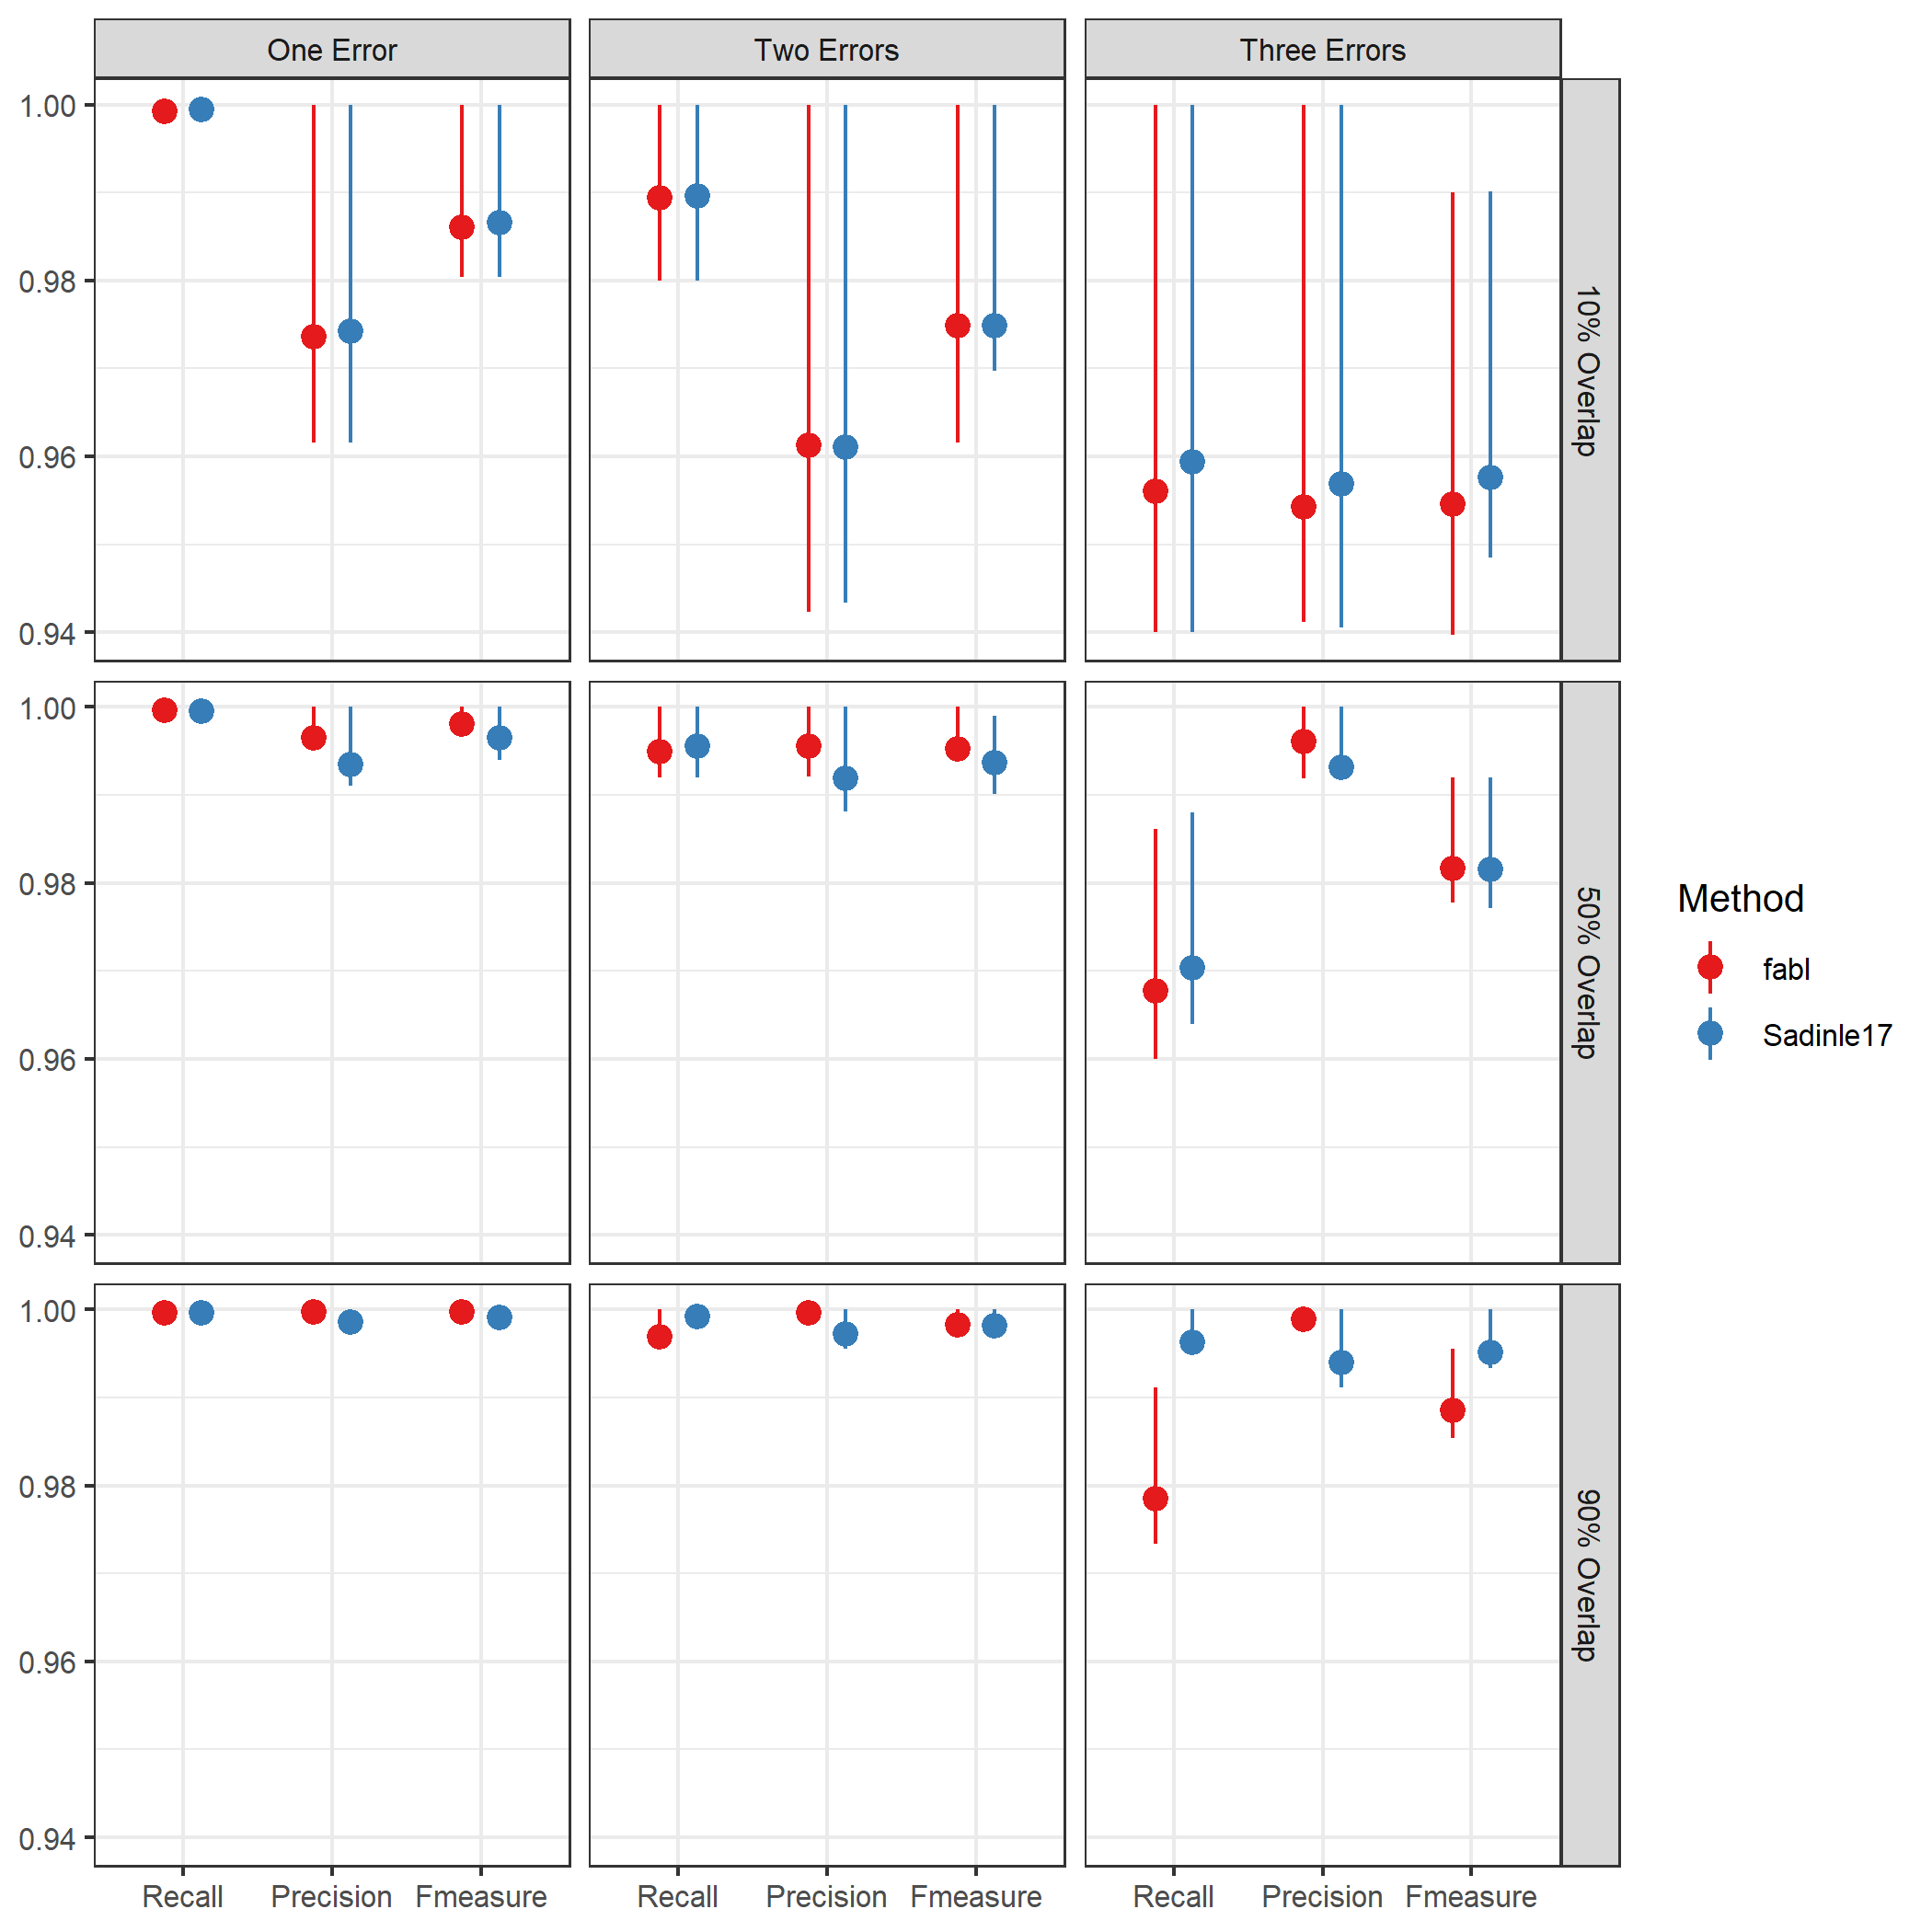
\includegraphics[width=0.6\textwidth]{../notes/figures/sadinle_sim_plot} 
	}
	
	\caption{Posterior means and credible intervals for accuracy metrics under the replication of simulation study from Sadinle 2017. For each level of overlap and each level of error, we have 100 paired sets of 500 records.}\label{fig:sadinle_simulation}
	
\end{figure}

\hypertarget{speed}{%
	\subsection{Speed}\label{speed}}

To demonstrate speed, we generate comparison vectors from pre-specified
distributions so that we can easily increase the size of the linkage
problem. Distributions are meant to emulate the behavior of similarity
scores across first name, last name, and day, month. For example, $u^{\text{month, 1}} = P(\text{Records have same birth-month | Nonmatch}) = \frac{1}{12}$. For simplicity, we
consider only exact matching, so a vector (1, 0) corresponds to
agreement and (0, 1) to disagreement. We simulate these data for
different values of \(n_A\) and \(n_B\), and compare the run-time of
\texttt{fabl} against \texttt{BRL}. Note that the number of unique
patterns \(P\) is bounded above by \(2^5 = 32\), a bound which is
consistently attained in the larger simulations.

We see that at low data size, \texttt{BRL} outperforms, but that
\texttt{fabl} is significantly faster at handling larger data. In
particular, run-time for \texttt{BRL} seems to grow quadratically (or
linearly with the size of both \(A\) and \(B\)) while run-time for
\texttt{fabl} seems to grow linearly (in the size of \(B\)).

\begin{table}[t]
	\centering
	\begin{tabular}{rrr}
		\hline
		& m & u \\ 
		\hline
		fname & $\left(\frac{19}{20}, \frac{1}{20}\right)$ & $\left(\frac{1}{100}, \frac{99}{100}\right)$ \\ 
		lname & $\left(\frac{19}{20}, \frac{1}{20}\right)$ & $\left(\frac{1}{100}, \frac{99}{100}\right)$ \\ 
		day & $\left(\frac{19}{20}, \frac{1}{20}\right)$ & $\left(\frac{1}{30}, \frac{29}{30}\right)$ \\ 
		month & $\left(\frac{19}{20}, \frac{1}{20}\right)$ & $\left(\frac{1}{12}, \frac{11}{12}\right)$ \\ 
		year & $\left(\frac{19}{20}, \frac{1}{20}\right)$ & $\left(\frac{1}{12}, \frac{11}{12}\right)$ \\ 
		\hline
	\end{tabular}
\caption{Distributions used for $m$ and $u$ probabilties in simulation studies}\label{fig:distributions}
\end{table}


\begin{figure}[ht]
	
	{\centering 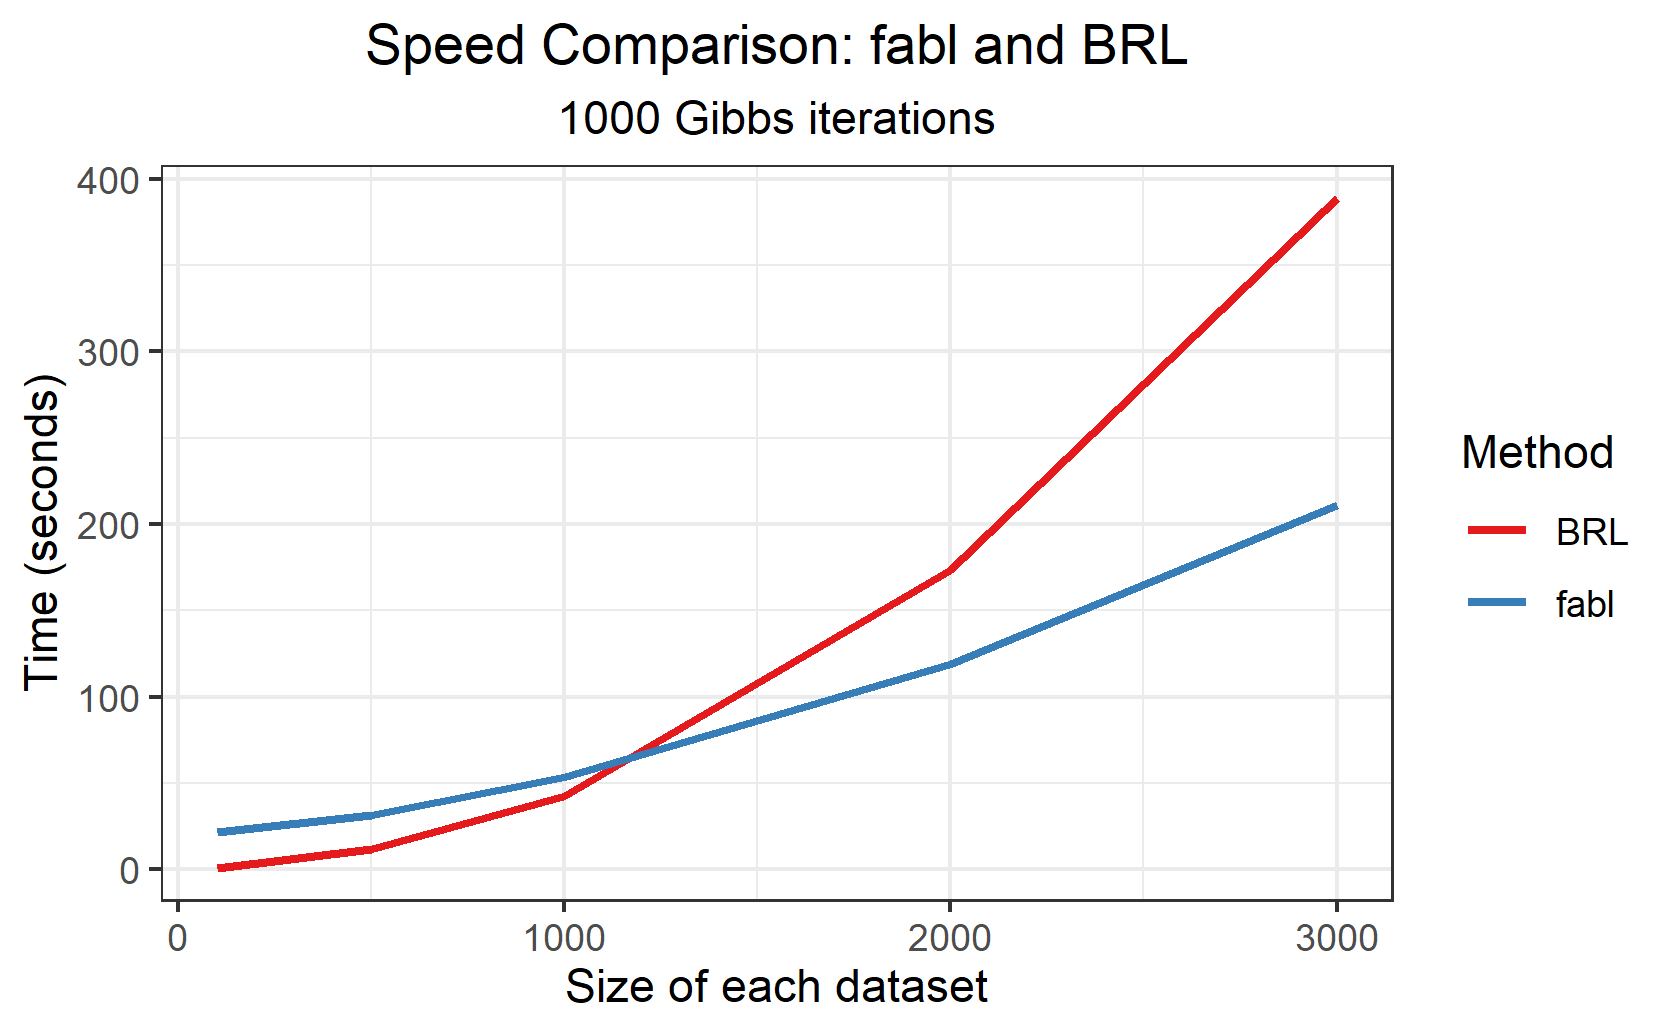
\includegraphics[width=0.6\textwidth]{../notes/figures/sadinle_speed_plot2} 
		
	}
	
	\caption{Run-time for BRL and fabl to run 1000 Gibbs iterations, including hashing step for fabl, for increasing values of both $n_A$ and $n_B$. We see near quadratic growth in runtime for BRL, and near linear growth for fabl.}\label{fig:speed1}
\end{figure}

The above discussion suggests that for fixed \(n_B\), computation time
should remain mostly constant with growing \(n_A\). Simulation study
suggests that this is true. In the plot below, fixing \(n_B = 500\), we
see linear growth for the run-time under \texttt{BRL} as \(n_A\)
increases, with much more static run-time under \texttt{fabl}. The
slight increases in run-time that we do see are due primarily to the
hashing step, which again can be run in parallel for large data.

\begin{figure}[t]
	
	{\centering 
\includegraphics[width=0.6\textwidth]{../notes/figures/speed_plot_fixed_nB} 
		
	}
	
	\caption{Run-time for BRL and fabl to run 1000 Gibbs iterations, including hashing step for fabl, with increasing $n_A$, and $n_B$ fixed at 500. We see linear growth in runtime for BRL, and near constant runtime for fabl.}\label{fig:speed2}
\end{figure}

We note here that \texttt{BRL} is coded in C, which makes for unfair
comparison against \texttt{fabl}, currently only built in R.
Additionally, although \texttt{fabl} is amenable to parallelization,
this simulation was run on a single core. Running \texttt{fabl} in C++
with paralellization for the hashing step and sampling the matching
status of the record pairs should lead to even more computational gains.

\hypertarget{scale}{%
	\subsection{Scale}\label{scale}}

% Assuming a 16GB personal machine, standard record linkage methods using all-to-all comparisons can only function on tasks where the matrix of comparison vectors $\Gamma$ is less than 8GB. In the context of the above simulation, each comparison vector contains four integers, collectively requiring 16 bytes of memory; assuming files of equal lengths, this means the largest linkage task possible is around $7000 \times 7000$. 
 
 In one final simulation, we demonstrate how partitioning and hashing the data through \texttt{fabl} method allows us undertake significantly larger linkage tasks We concatenate two sets of 40 simulated datasets from the Sadinle simulation to create two larger files, each of 20,000 records. Working on one machine, we sequentially compare records across chunks, hash results, and then synthesize summary statistics for the entire simulation. Under standard Fellegi Sunter procedures, this would require 400,000,000 comparison vectors, each consisting for four integers, resulting a final comparison matrix about 6.4 GB in size. 
 
 For simplicity, we partition one dataset into 20 smaller chunks, and leave the second dataset fully intact. We then compare records, hash results, and then synthesize summary statistics for all 20 chunk comparisons. The resulting data object is only 90 MB, about 1\% the size of the object required under the standard method. Excecuted sequentially, these comparisons and the Gibbs sampler take about one hour to run; using distributed computing, it could be completed much faster. This simulation achieved 96.5\% recall and 97.7\% precision, with an overall F-measure of 97.1\% F-measure. The reader will note that this slightly worse performance than witnessed in the smaller simulation studies; this is expected because it is naturally more difficult to link more files with the same amount of information. With more linkage fields \texttt{fabl} maintains the high accuracy seen above. 
 
 

\section{Case Studies}
\label{sex:case-studies}

We now demonstrate the power of our method through a case study of documented identifiable deaths (DID) from the El Salvadoran Civil War. Though the data files used here are small, this study shows how the computational complexity of \texttt{fabl} depends on the number of unique agreement patterns, and how significant computational gains can be achieved by simplifying the construction of the comparison vectors. Secondly, the case study reveals the impact of independently sampling $Z_j$ rather than strictly enforcing one-to-one matching as done by \texttt{BRL}. 

%The second case study is the National Long Term Care Survey (NLTCS), a much larger linkage tasks which \texttt{BRL} is unable to complete but which we complete with \texttt{fabl} with relative ease. 

\subsection{El Salvadoran Civil War}
\label{el_salvador}

The country of El Salvador was immersed in civil war from 1980 to 1991,
and throughout the time, several organizations attempted to document
casualties of the conflict. When estimating the total number of
casualties, one cannot simply sum the numbers recorded by each
organization, as it is likely that the same individuals are recorded in
multiple casualty lists. To obtain a more accurate estimate of the
casualties then, we follow Sadinle's 2017 paper and link records of El
Salvadoran civilian casualties from two sources: El Rescate - Tutela
Regal (ERTL) and the Salvadoran Human Rights Commission (CDHES, by its
acronym in Spanish). The ERTL dataset consists of digitized reports that
had been published throughout the conflict. The CDHES dataset consists
of casualties that had been reported directly to the organization, and
later digitized.

There are several challenges with working with such data. Firstly, both
datasets have been automatically digitized, which inherently leads to
some degree of typographical error. Secondly, the CDHES records are all
second hand accounts reported by individuals, which can result in
additional errors. Lastly, the only fields recorded are given name, last
name, date of death, and place of death; it is relatively common for a
parent and child to share the same given name, resulting in
indistinguishable records for two different individuals. This last point
nearly breaks the earlier mentioned assumption that there are no
duplicates within files, and reveals a key difference between
\texttt{BRL} and our proposed method.

We only utilized records with nonmissing entries for given and last
name, results in \(n_A = 4420\) files in CHDES and \(n_B = 1323\) files
in ERTL. The names were standardized to account for common misspellings
in the Spanish language, and then compared using a modified Levenstein
distance to account for the fact that second names are often omitted.
Place of birth is recorded by municipality and department within that
municipality; however, since department was missing in 95\% of records
in CHDES and 80\% of records in ERTL, we excluded it from our linkage
process. Thus we conduct linkage using given name, last name,
municipality, and day, month, and year of death. We again use flat
priors for the \(\mathbf{m}\) and \(\mathbf{u}\) parameters.

\begin{figure}[t]
	
	{\centering 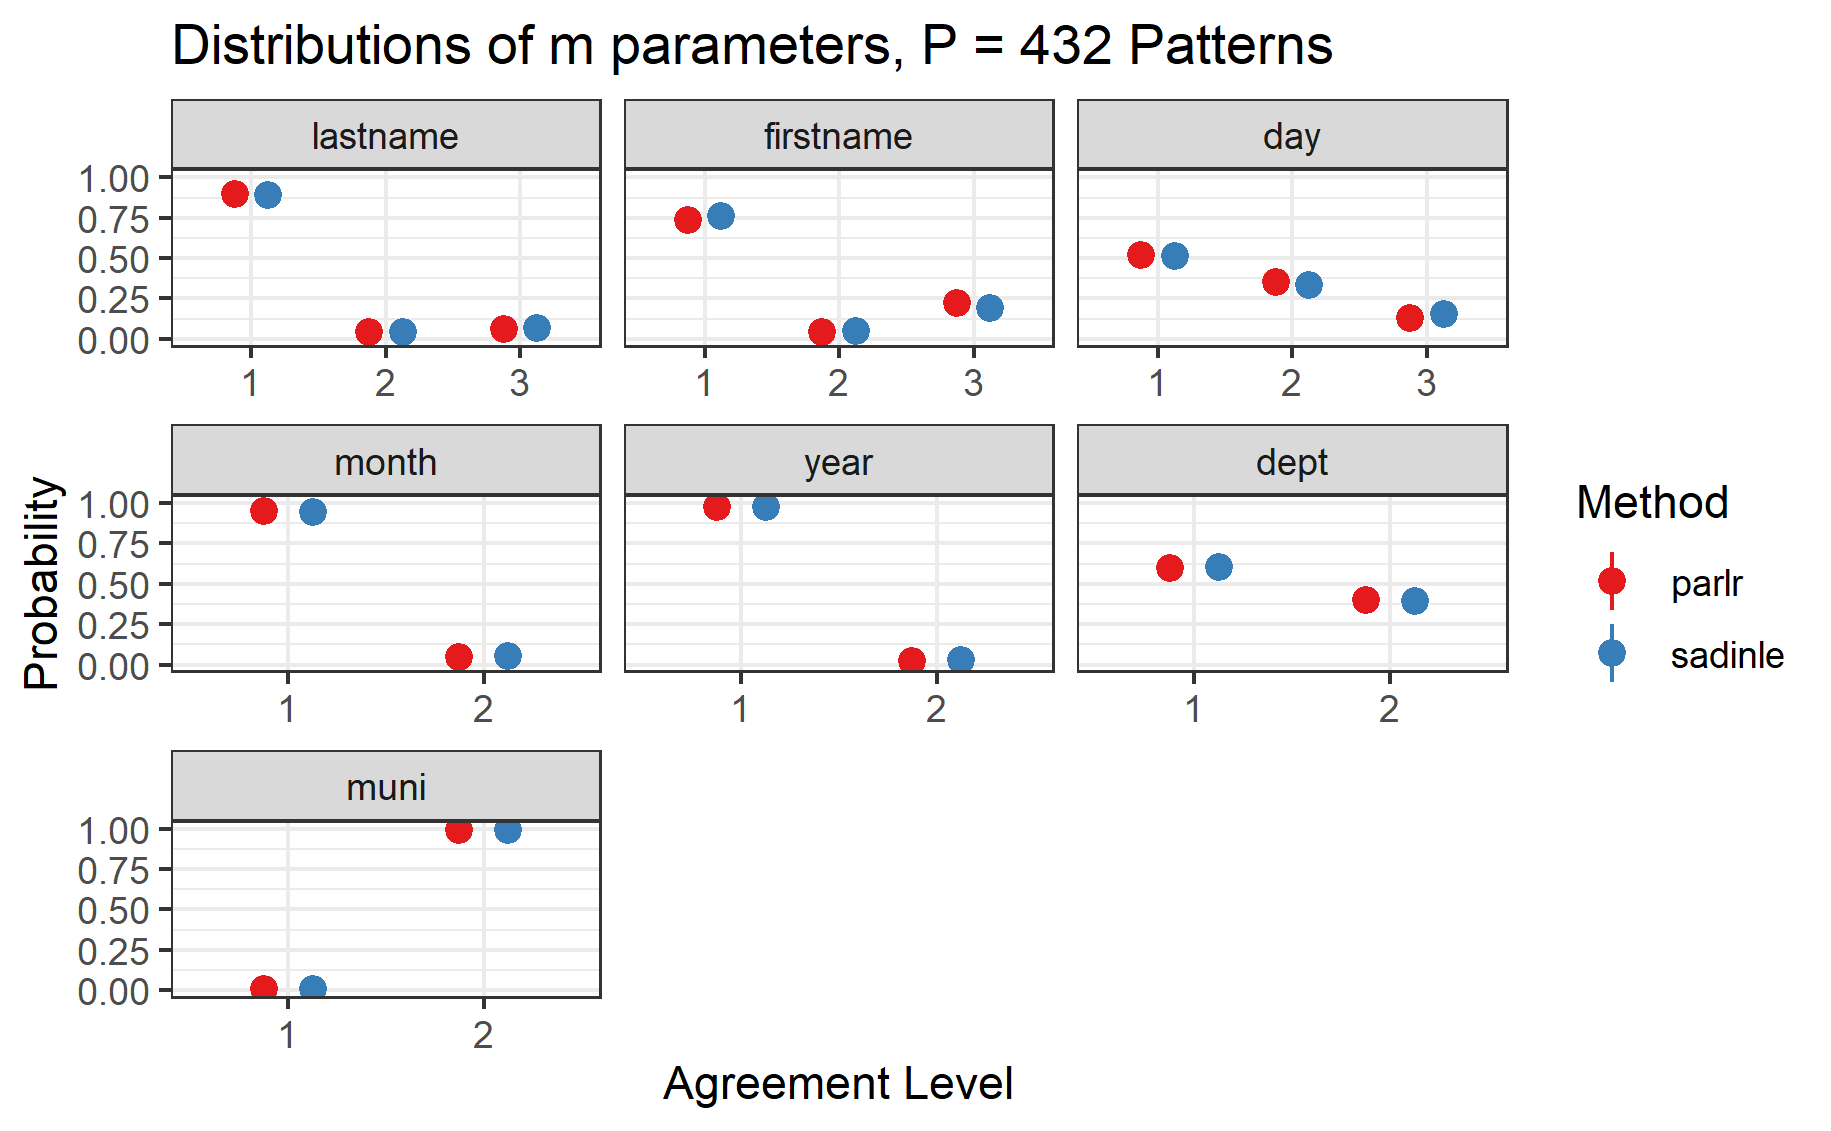
\includegraphics[width=0.6\textwidth]{../notes/figures/el_salvador/m_posterior_smallP} 
		
	}
	
	\caption{Posterior estimates of m parameters with 95\% credible intervals}\label{fig:m-and-u}
\end{figure}

To mirror the original implementation, we constructed the comparison
vectors using 4 levels of agreement for each field, according to the
thresholds provided in Figure XX. This took 422 seconds for our proposed
method and 240 for \texttt{BRL}. However, we observed that posterior
distributions of several levels of the \(\mathbf{m}\) and \(\mathbf{u}\)
parameters were nearly identical, and that of the
\(4^5 \times 2 = 2048\) possible agreement patterns, only 1173 are
realized in the data. This leads us to believe that such high number of
agreement levels creates unnecessary distinctions in the data and makes
the comparison vectors less interpretable. Therefore we re-ran our
analysis with fewer agreement levels for each field (see Figure XX), and
obtained analogous results. With 216 possible agreement patterns, 159
were realized in the data, and our proposed method became much faster,
finishing in 124 seconds. Meanwhile \texttt{BRL} took 239 seconds,
relatively unchanged from the first implementation. This demonstrates
the way that the computational complexity of our method depends on the
number of unique agreement patterns, and how significant computational
gains can be made by simplifying the construction of the comparison
vectors. We also note that estimates of the \(\mathbf{m}\) and
\(\mathbf{u}\) parameters under each method are very similar, as shown in
Figure~\ref{fig:m-and-u}.

\paragraph{Violations of One-to-One Matching} Figure~\ref{fig:overlap-plot} shows the posterior distribution for \(D\), the number of
duplicates found across file for both \texttt{fabl} and \texttt{BRL}. We
see that \texttt{fabl} consistently overmatches within each Gibbs
iteration when compared to \texttt{BRL}, which is to be expected because
\texttt{BRL} explicitly prevents matches that violate one-to-one
matching throughout the entire sampler. Most of such matchings are due
to the randomness in the sampling procedure, and they occur sporadically
throughout the sampler in such a way that does not measurably influence
the eventual Bayes estimate.

\begin{figure}[t]
	
	{\centering 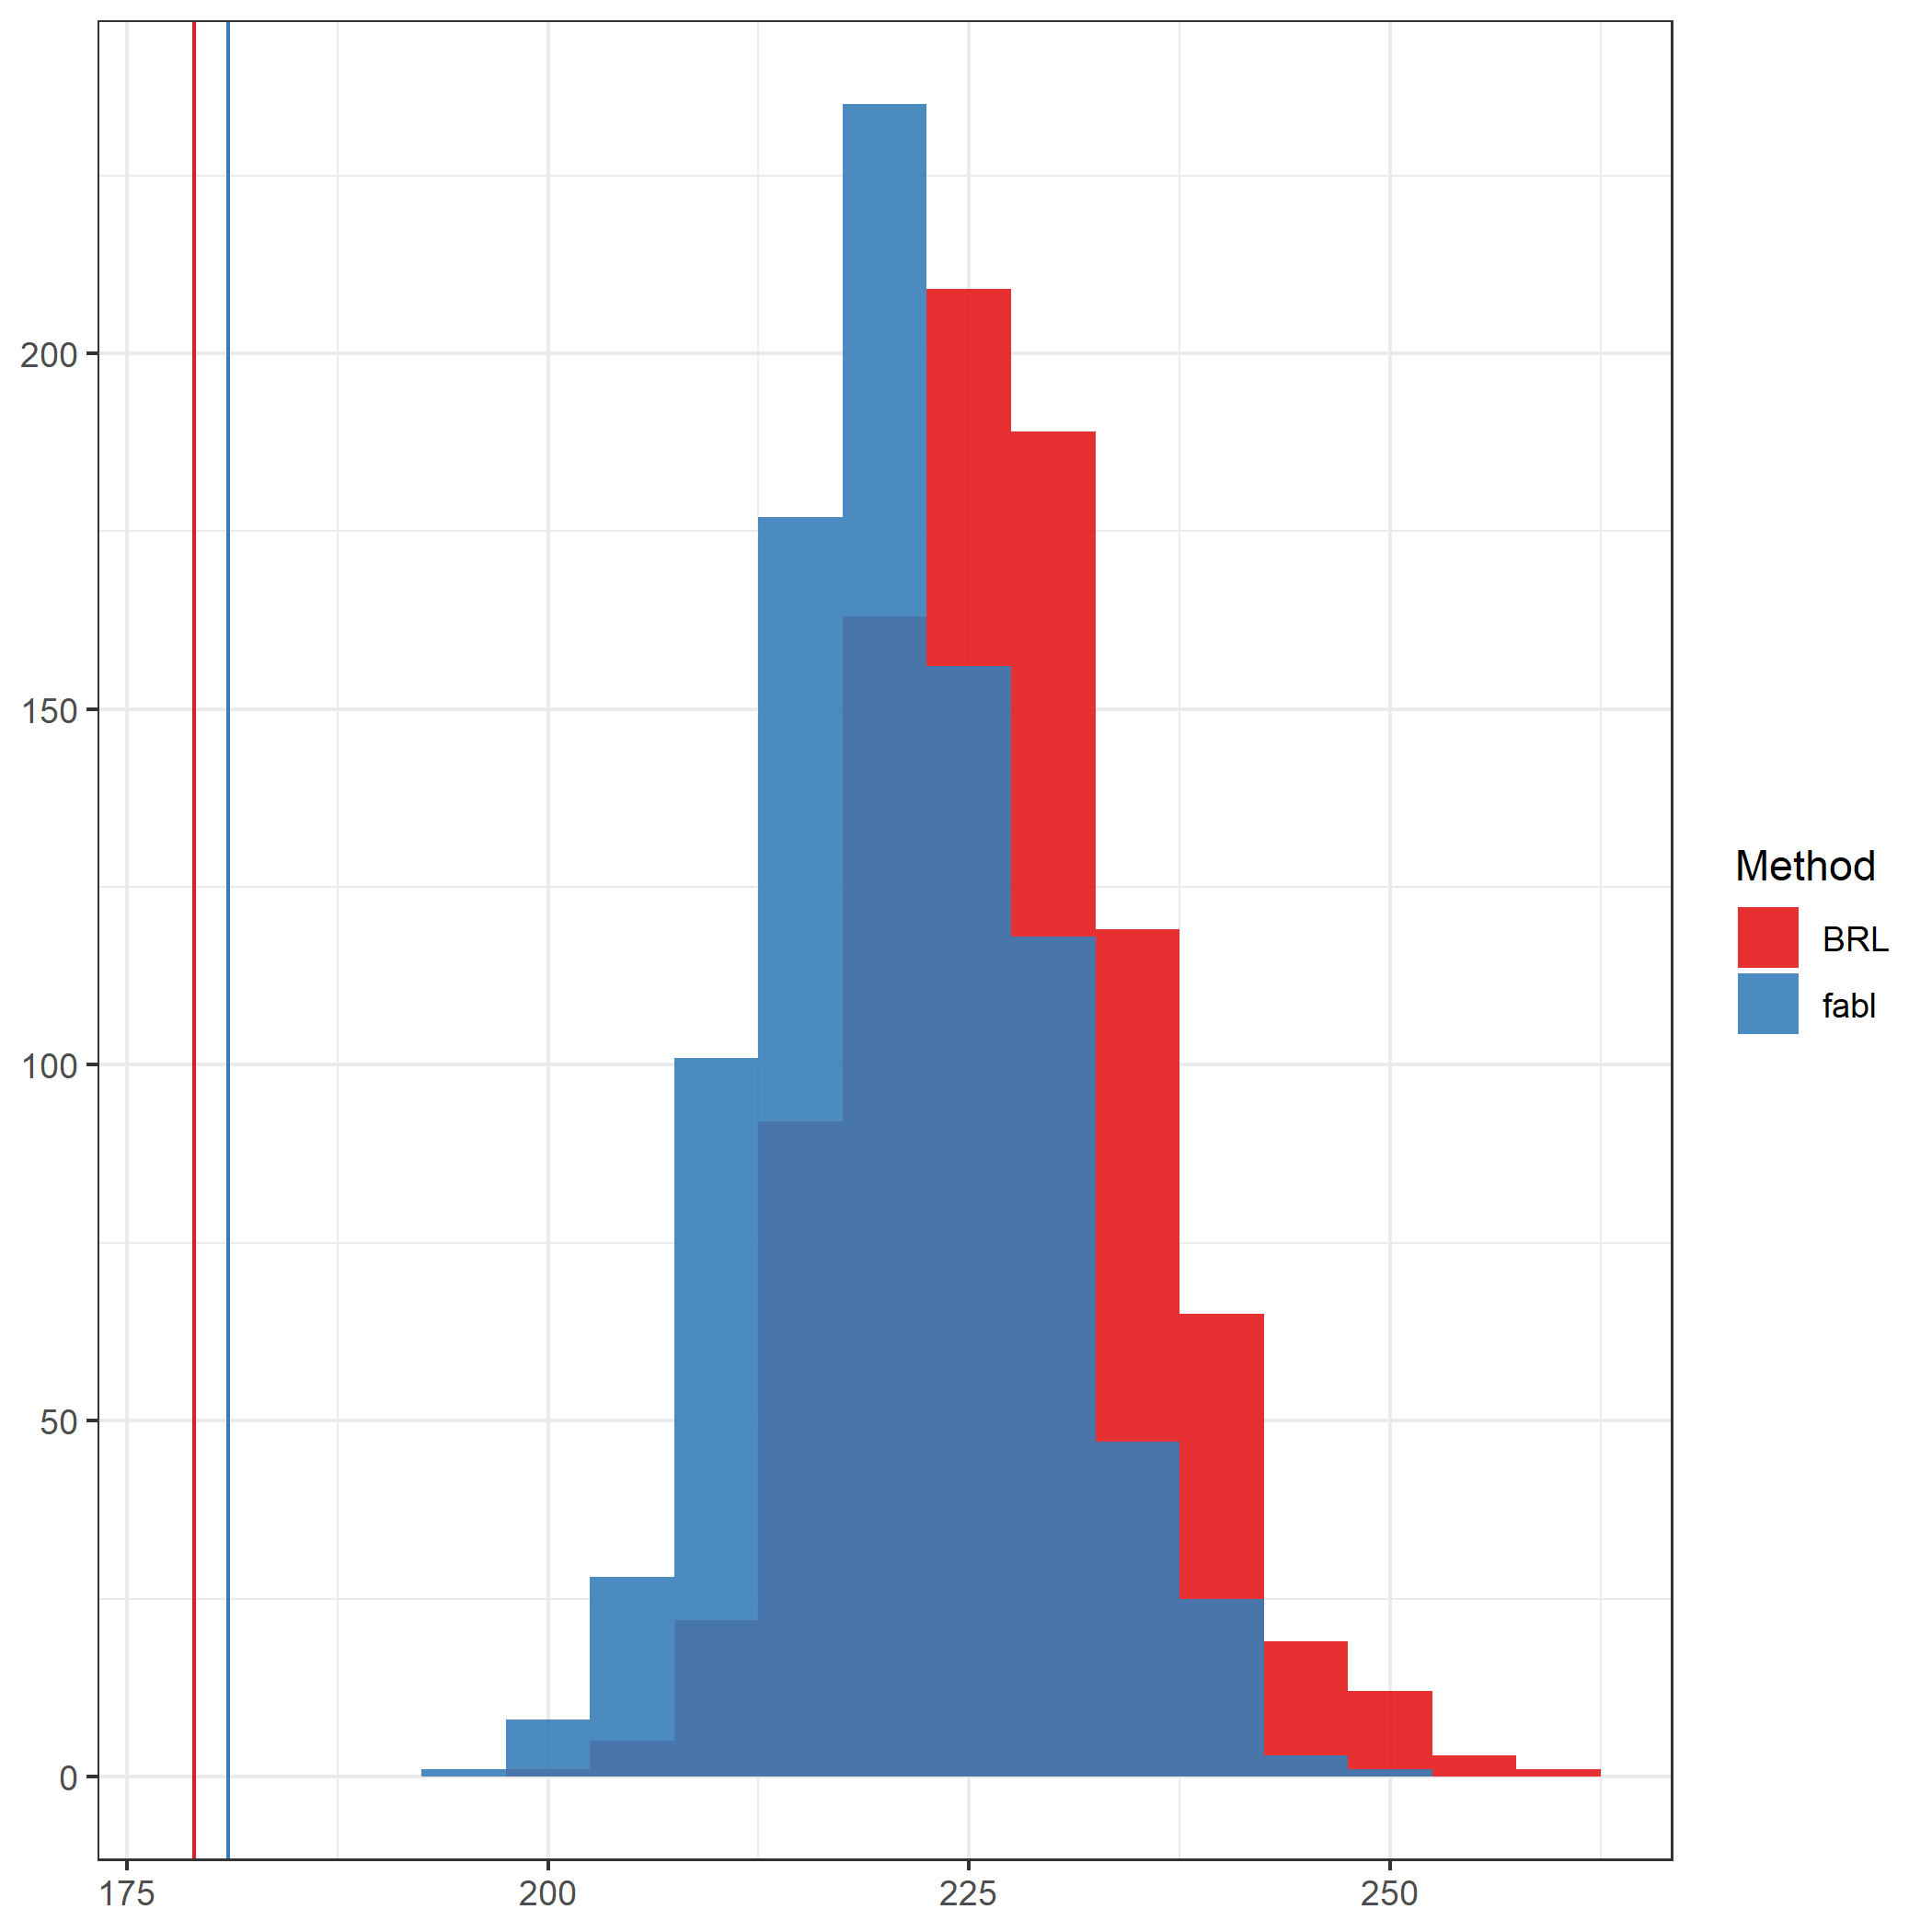
\includegraphics[width=0.6\textwidth]{../notes/figures/el_salvador/overlap_distribution_smallP_bayes} 
		
	}
	
	\caption{Posterior distribution of overlap across the two files. The solid lines show the Bayes estimate for the amount of overlap, and the dashed line is the Bayes estimate under fabl before resolving violations of one-to-one matching}\label{fig:overlap-plot}
\end{figure}

Overall, both methods presented similar results. \texttt{fabl} yielded
an initial Bayes estimate of 195 matches found across files, and after
resolving matches that violated one-to-one requirements, yielded 180
matches across files. This is acceptably close to the 181 matches found
by \texttt{BRL}. The main reason for this discrepancy is the difference
in how each model handles situations in which one file in \(B\) has
multiple plausible matches in \(A\).

\begin{figure}[t]
	
	{\centering 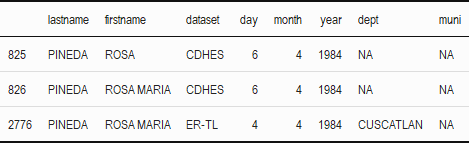
\includegraphics[width=0.6\textwidth]{../notes/figures/el_salvador/rosa_records} 
		
	}
	
	\caption{Example of linkage situation with multiple plausible matches}\label{fig:rosa-maria}
\end{figure}

\begin{figure}[t]
	
	{\centering 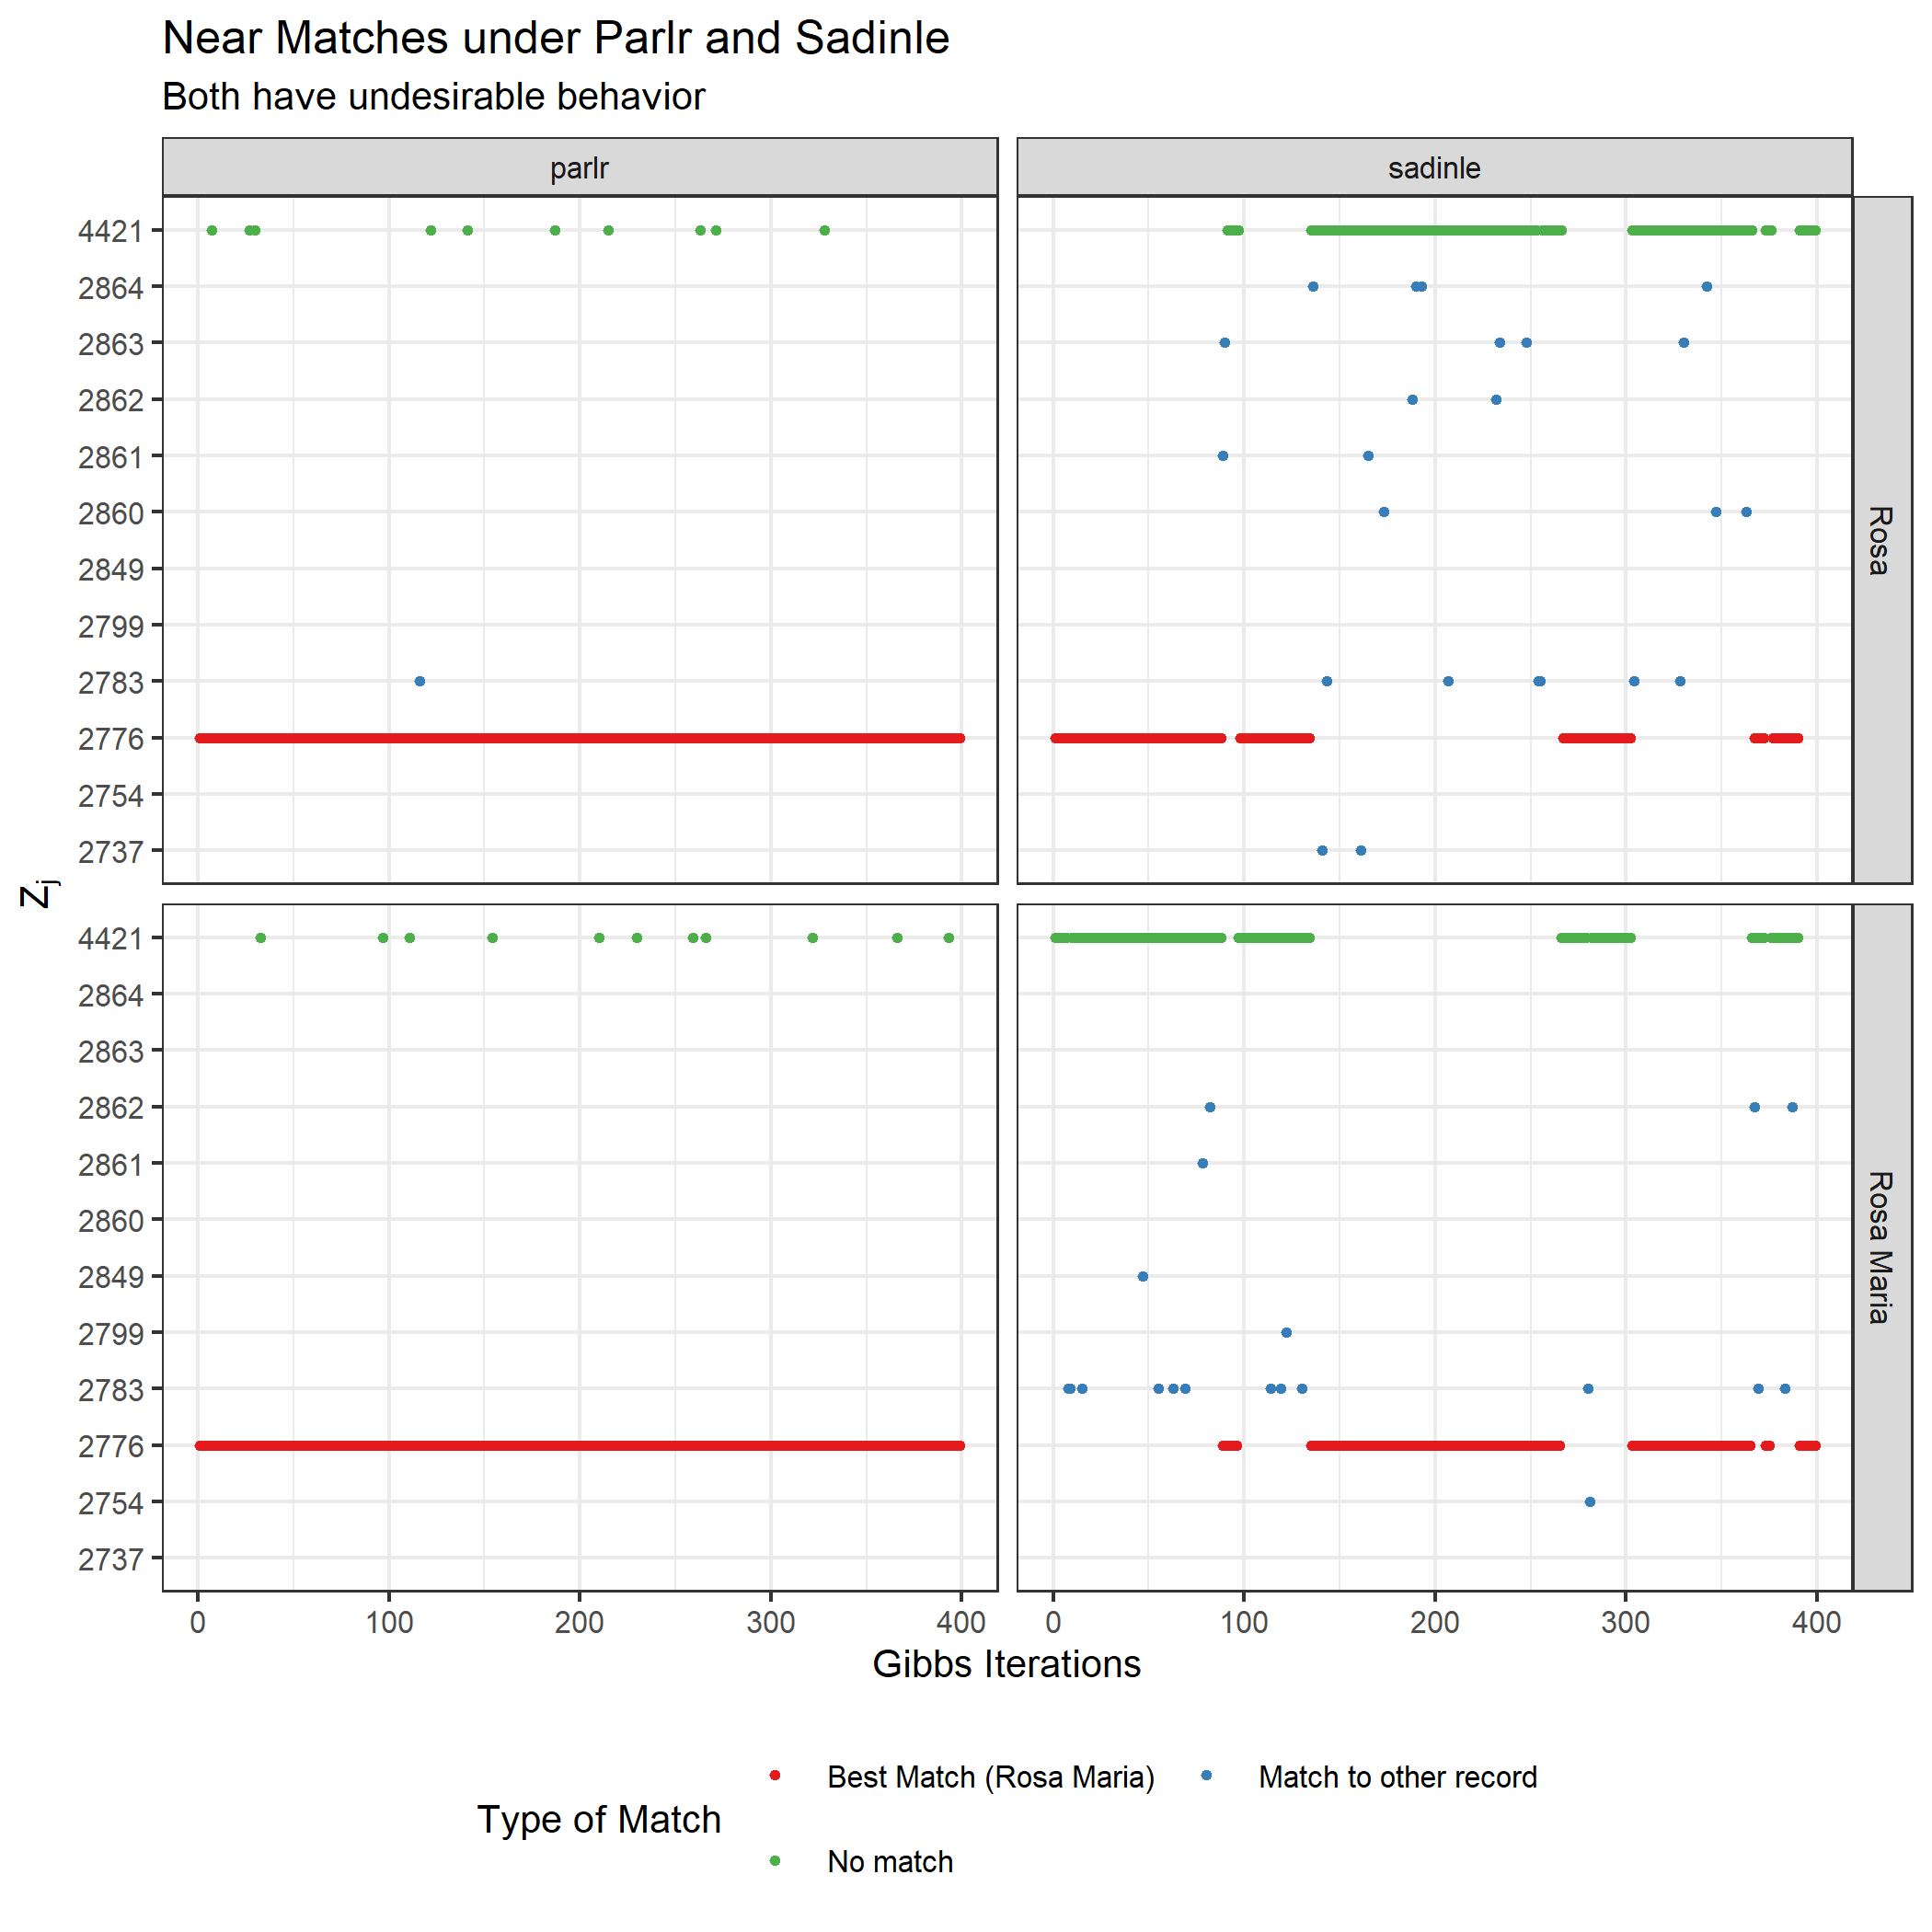
\includegraphics[width=0.6\textwidth]{../notes/figures/el_salvador/bad_mixing} 
		
	}
	
	\caption{Gibbs sampling in situation with multiple plausible matches.}\label{fig:mixing-plot}
\end{figure}

The records shown in Figure~\ref{fig:rosa-maria} provide one such instance. Note these
records present a near violation of our assumption that there are no
duplications within files; we continue to assume that records 825 and
826 in ERTL correspond to different individuals, but their records are
nearly identical. Additionally, using the modified Levenstein distance
from Sadinle 2017, the comparison vectors \(\gamma_{2776, 825}\) and
\(\gamma_{2776, 826}\) are exactly identical.

Figure~\ref{fig:mixing-plot} shows the values that \(Z_{825}\) and \(Z_{826}\) take on
throughout the Gibbs sampler, and demonstrates how each method handles
this situation. Under \texttt{fabl}, both records in \(B\) match to the
same record in \(A\) throughout the Gibbs process, creating consistent
violations of one-to-one matching. Under \texttt{BRL}, the Gibbs process
creates one matching configuration stays there for a while. However, if
one pair ``unmatches,'' then the other record has a chance to latch on.
Then, the Gibbs process is stuck with that matching status for a while,
resulting in a Gibbs process with poor mixing. Additionally,
\texttt{fabl} allows the modeler to inspect records with multiple
plausible matches, and if they desire, to then choose the record pairing
with the highest posterior probability. \texttt{BRL} in contrast, in
strictly enforcing one-to-one matching throughout the sampler, can lead
to situations where none of the plausible matches reach the threshold to
be identified through the Bayes estimate.

%\subsection{National Long Term Care Survey}
%\label{nltcs} 
%
%The National Long Term Care Survey is a longitudinal study to track changes in health among Medicare recipients. It was conducted approximately every five years, and we concern ourselves here with linking records from years 1982 and 1989. The data only contains day, month, and year of birth, sex, state the individual lives in, and regional office. State and regional office have been anonymized, presented as numbers instead of their actual values. We construct the comparison vectors using only binary exact matching for each field, since there is no straightfoward way to incorporate partial matching in this context. The 1982 file contains $n_A = 20485$ records, 1989 file contains $n_B = 17466$ files, and the six linkage fields induces $2^6 = 64$ possible unique agreement patterns. We note that linkage quality is bound to be quite weak for many potential matches with such a large number of records and such limited identifying information.  
%
%With such large files, performing all-to-all comparisons under the original Fellegi-Sunter framework is infeasible. Indeed, this would require nearly 400 million comparison vectors, each containing 6 integer comparisons; the resulting data object would contain over 2 billion integers, and would require approximately 16 GBs of memory to hold. Instead, we take the partitioning approach reviewed in \ref{data-representation-hashing-and-storage}, and split each dataset into 10 smaller datasets. We use parallel computing on cluster service create the comparison vectors for each pair of data chunks, hash the results, and compress in size through storage efficient indexing. We then aggregate the results, creating a data object of just 87 MB, and proceed with the Gibbs Sampler. 
%
%Were a personal computer able to hold the 16 GB data object required by the direct approach, the Gibbs sampler under \texttt{BRL} would be tortuously slow, with computational complexity $O(n_A \times n_B \times F)$ where $n_A = 20485$. However, under \texttt{fabl} the sampler has complexity $O(P \times n_B \times F)$ where $P = 64$, so 1000 iterations of the Gibbs sampler are completed in just XX seconds. Posterior analysis yields an initial estimate of 9991 individuals linked across the the two datasets, and 8895 individuals linked once conflicts are resolved to ensure one-to-one matching. 
%
%Lastly, we comment on the significance of conducting this linkage without the use of deterministic blocking. With previous methods, one could link these two records by blocking on a certain field, and running separate Gibbs samplers on each of the separate blocks. This strategy drastically improves computation since it significantly reduces the number of comparison vectors that need to be formed and uses smaller data objects throughout the sampler. However, this computational savings comes at the cost of missing potential links, specifically in cases where the blocking variable is recorded in error. In this case, 62 of the matched pairs exhibit a disagreement in sex, 17 exhibit a disagreement in state, and 39 exhibit a disagreement in regional office. We have no way to verify that the matches found under \texttt{fabl} are indeed correct, so it is possible that matches found with such disagreements are false positives. Even if not, the modeler may conclude that, for example, 17 missed matches are a small price to pay to be able to block on state and run 50 smaller, independent linkage procedures. However, \texttt{fabl} allows the modeler to make this choice for themselves, rather than being forced to do so for computational reasons. Additionally, by running on the Gibbs sampler the entirety of both files, we achieve $m$ and $u$ parameters that are interpretale for the entire study, rather than separate parameters for each block. Although these $m$ and $u$'s are often regarded as nuisance parameters in the record linkage literature, \texttt{fabl} allows for study of these parameters that has been been possible before. 

\section{Discussion}
\label{discussion}

We have presented a method for Bayesian record linkage that is feasible
for large datasets. In particular, our hashing procedure and model
assumptions allow for a linkage procedure whose computational complexity
does not scale with the size of the larger dataset, making this method
particularly powerful in linking records when one datafile is
substantially smaller than the other.

In our case study, we included an exploration of how to conduct record
linkage when modeling assumptions are not met in practice. We explored
``one-to-many'' scenarios in which one record in \(A\) has multiple
plausible matches in \(B\), and showed how both \texttt{fabl} and
\texttt{BRL} demonstrated undesirable qualities. Other issues arise
under ``many-to-one'' scenarios, where one record in \(B\) has multiple
plausible matches in \(A\), and ``many-to-many'' scenarios in which
there is duplication both across and within datasets. Tuning
\texttt{fabl} for use in these scenarios is one potential avenue for
future work.

\bigskip

\section{Appendix}
\label{sec:appendix}

\begin{figure}[t]
	
	{\centering 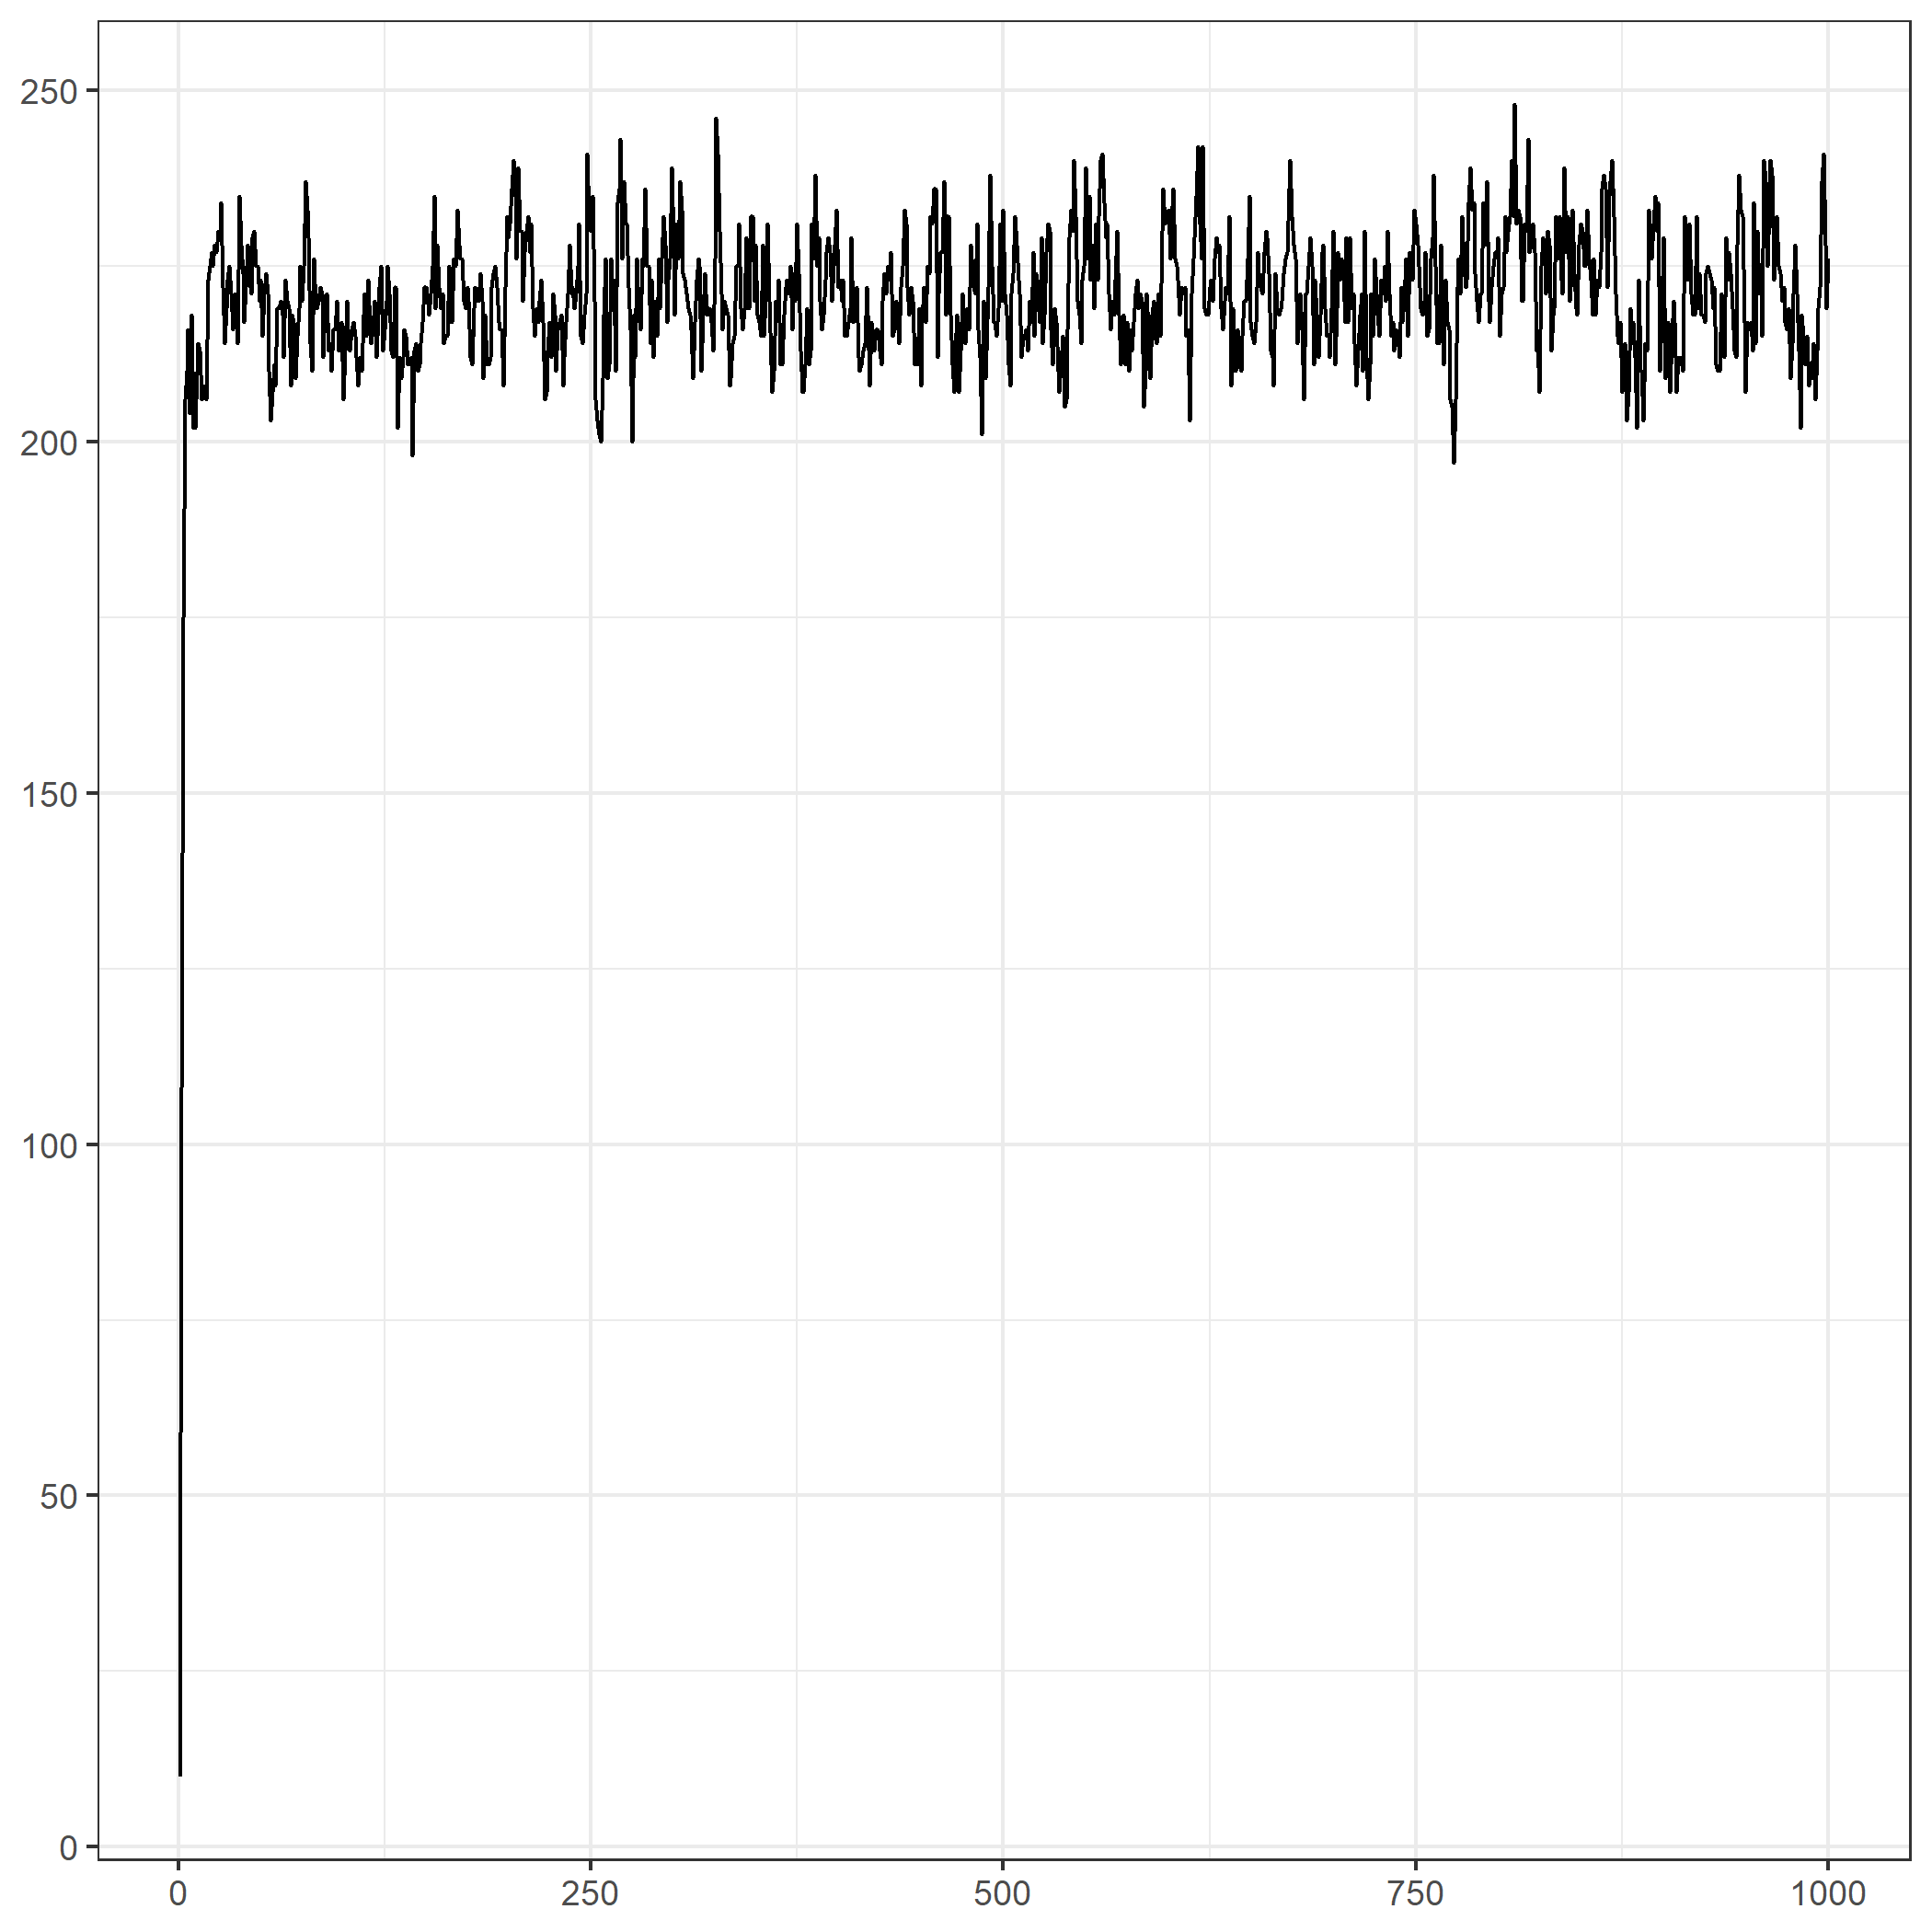
\includegraphics[width=0.6\textwidth]{../notes/figures/el_salvador/overlap_trace} 
		
	}
	
	\caption{Traceplot for number of matches found across datasets in El Salvador case study}\label{fig:overlap_trace}
\end{figure}

\begin{figure}[t]
	
	{\centering 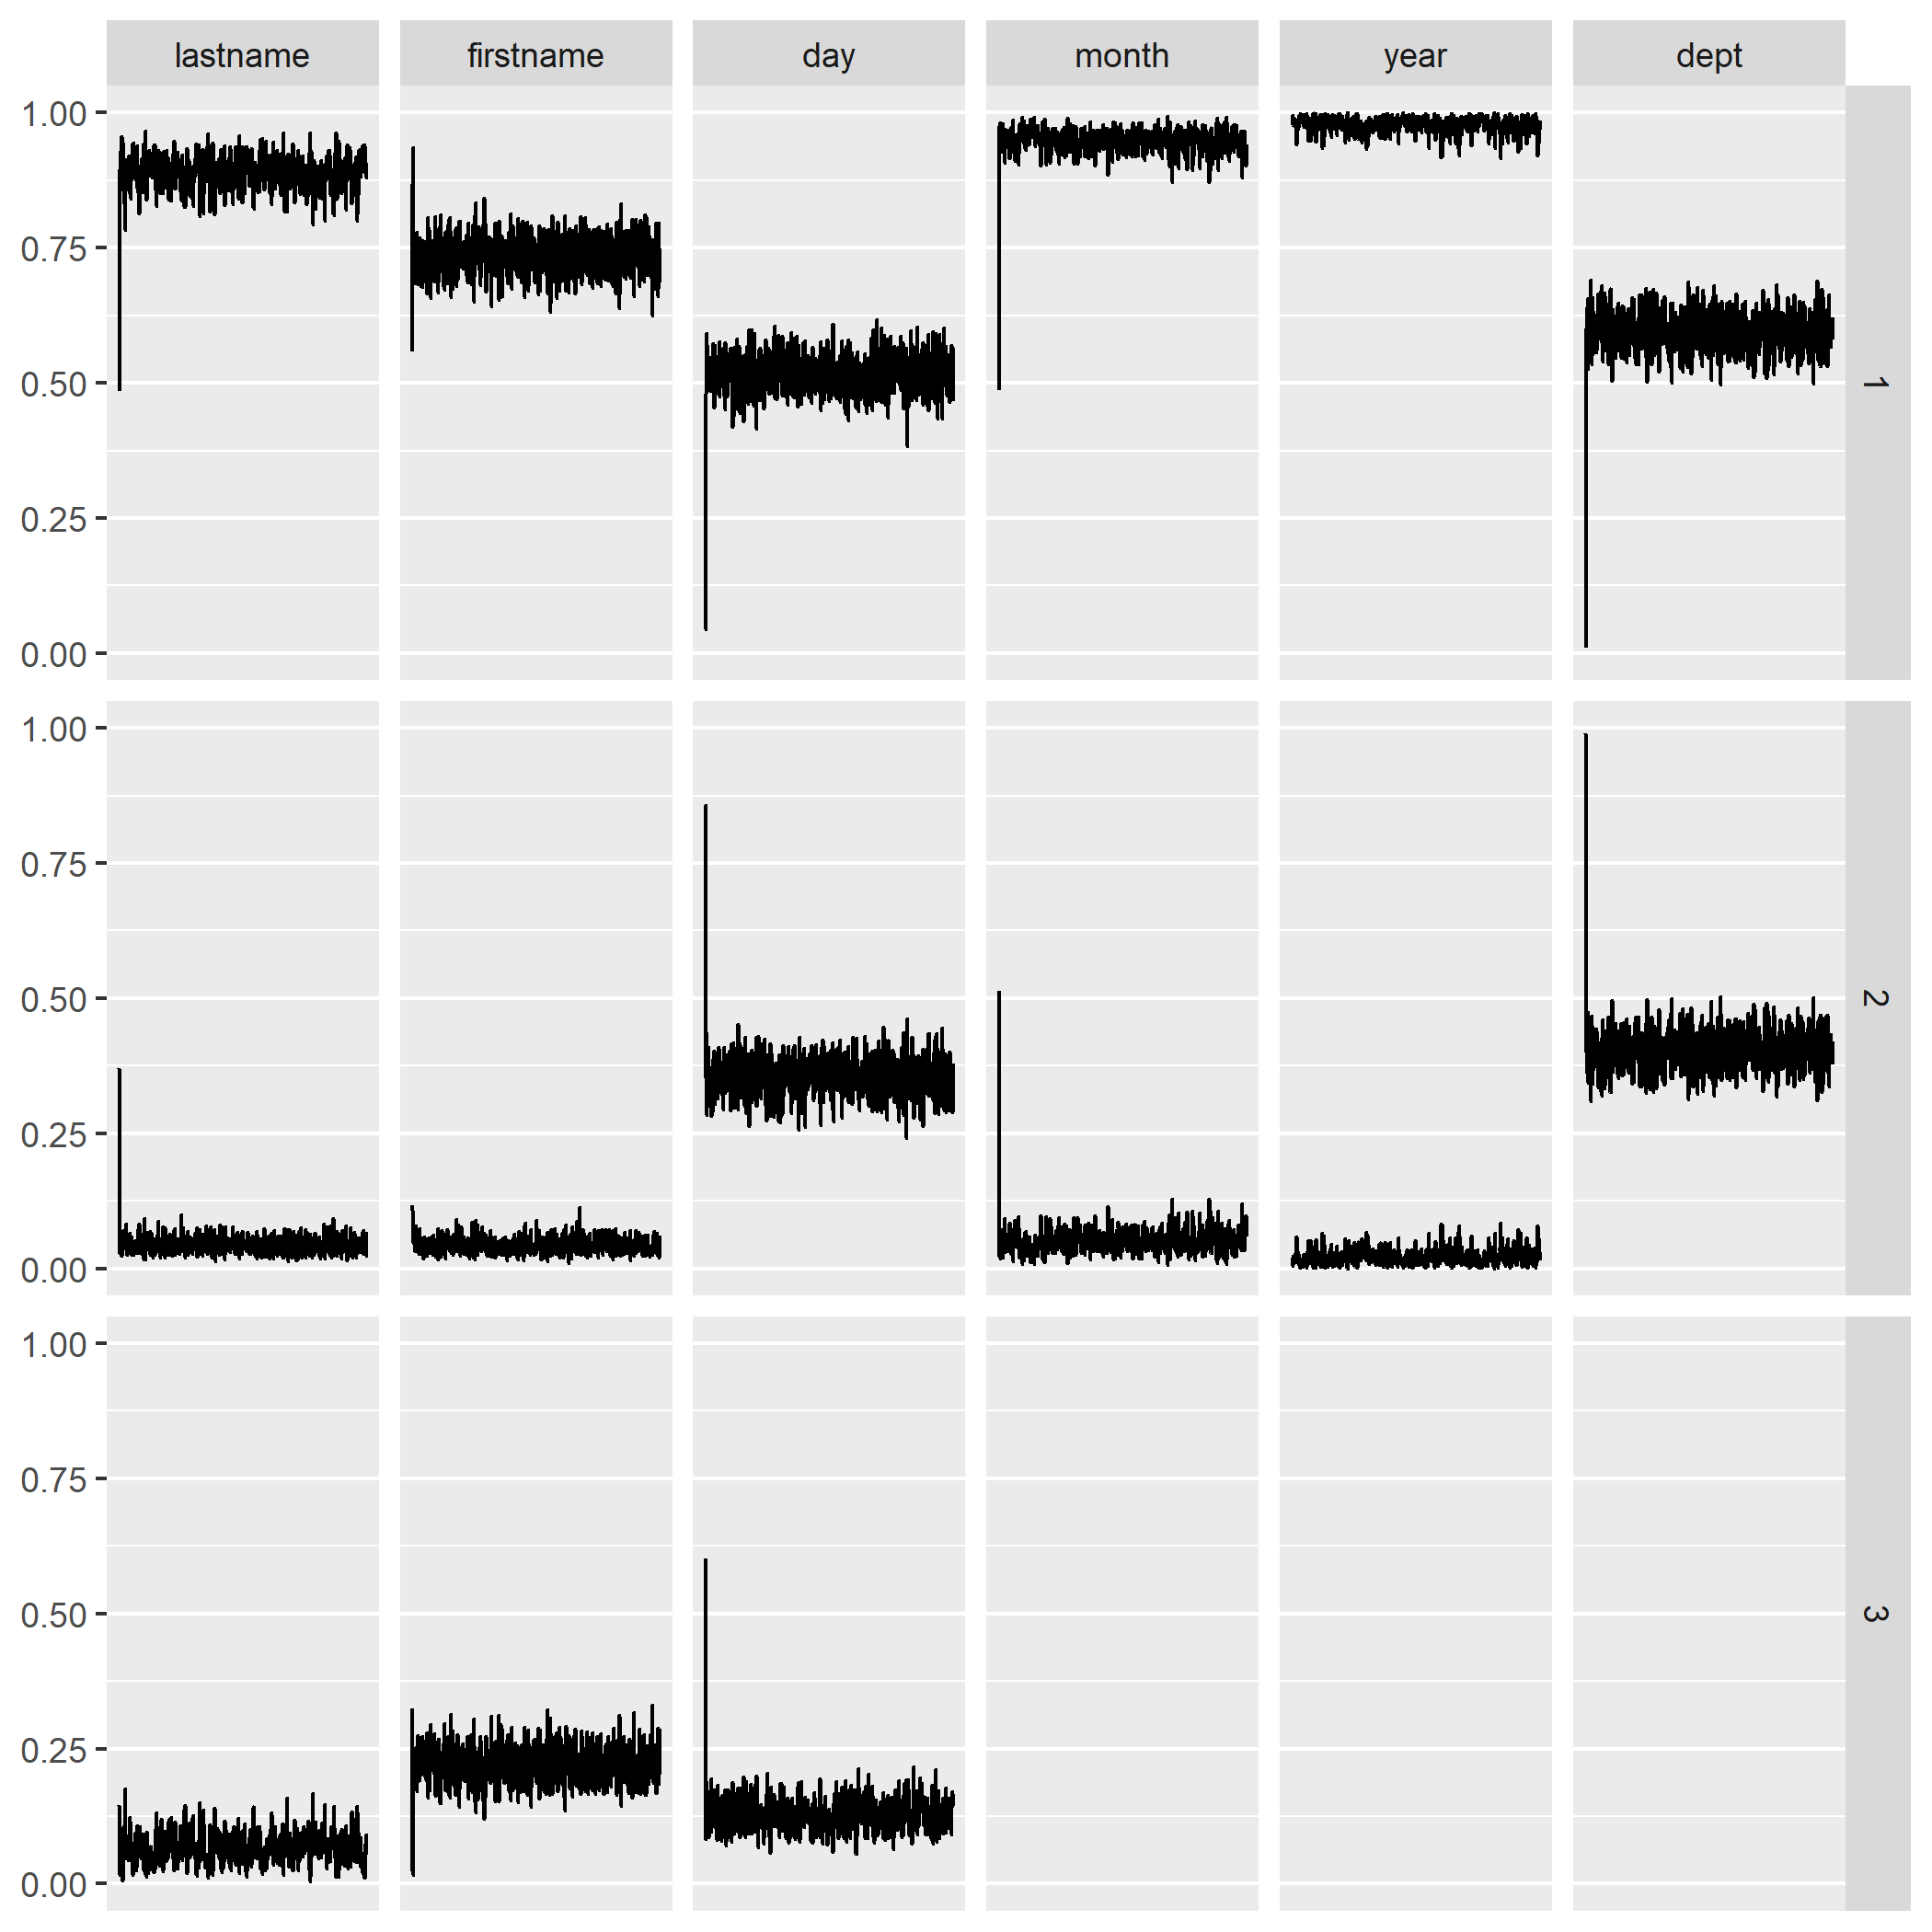
\includegraphics[width=0.6\textwidth]{../notes/figures/el_salvador/m_trace} 
		
	}
	
	\caption{Traceplot for m parameter in El Salvador case study}\label{fig:m_trace}
\end{figure}

\begin{figure}[t]
	
	{\centering 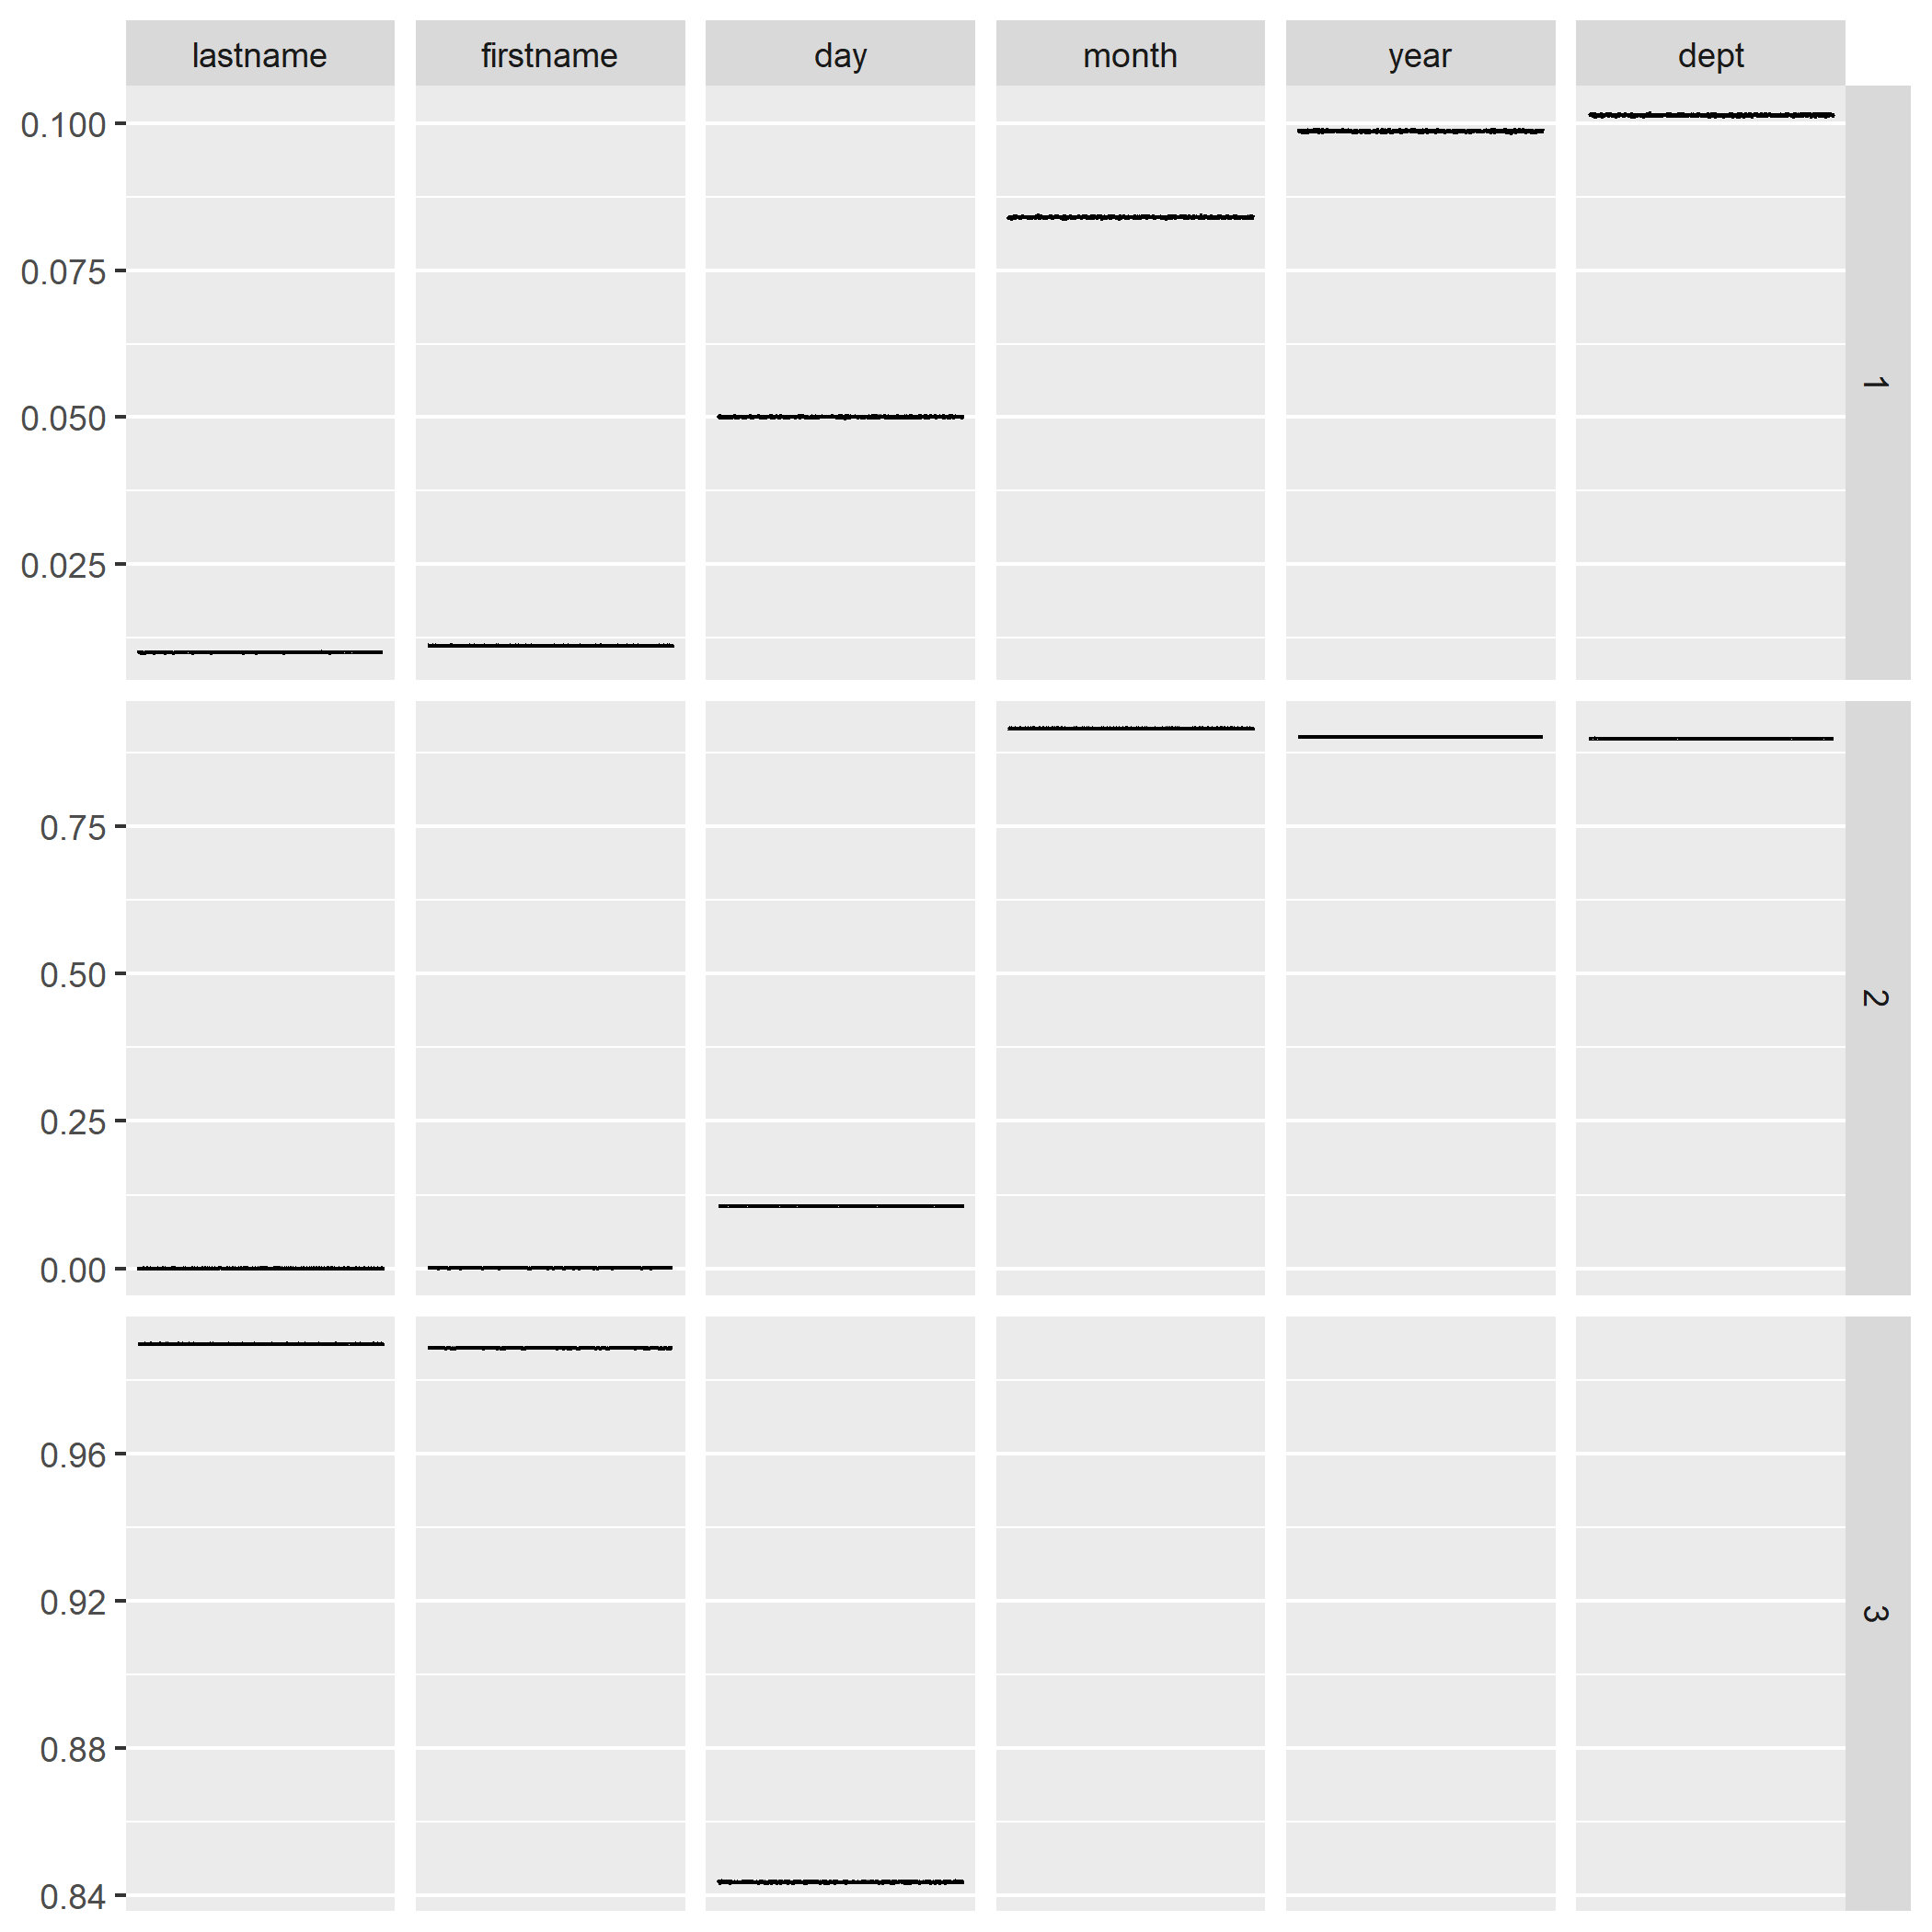
\includegraphics[width=0.6\textwidth]{../notes/figures/el_salvador/u_trace} 
		
	}
	
	\caption{Traceplot for u parameter in El Salvador case study}\label{fig:u_trace}
\end{figure}

\bigskip

\bibliographystyle{jasa}
{
\footnotesize
\bibliography{references}
}

\end{document}
